% Paper draft for FPGA 2013
\documentclass{acm_proc_article-sp}
\usepackage{graphicx}
\usepackage{multirow}
\usepackage[caption=true,font=footnotesize]{subfig}
\usepackage{dblfloatfix}
\usepackage{algorithmic}
\usepackage{algorithm}
\usepackage{xspace}
\usepackage{url}
\usepackage{bm}
%\renewcommand{\topfraction}{0.5}
%\renewcommand{\dbltopfraction}{0.5}

\renewcommand\floatpagefraction{.9}
\renewcommand\topfraction{.9}
\renewcommand\bottomfraction{.9}
\renewcommand\dbltopfraction{.9}
\renewcommand\textfraction{.1}   
\setcounter{totalnumber}{50}
\setcounter{topnumber}{50}
\setcounter{bottomnumber}{50}

\newcommand{\eqnref}[1]{(\ref{#1})}
\newcommand{\figref}[1]{Figure~\ref{#1}}
\newcommand{\algref}[1]{Algorithm~\ref{#1}}
\newcommand{\secref}[1]{Section~\ref{#1}}
\newcommand{\tabref}[1]{Table~\ref{#1}}
\newcommand{\autoesl}{AutoESL\xspace}
\newcommand{\tabincell}[2]{\begin{tabular}{@{}#1@{}}#2\end{tabular}}

\usepackage{etoolbox}
\makeatletter
\patchcmd{\maketitle}{\@copyrightspace}{}{}{}
\makeatother
\graphicspath{{./figures/}}

\begin{document}

\title{Automatic Overlay Customization For High-Productivity Nested Loop Acceleration On FPGA}

\numberofauthors{1}
 \author{
% % 1st. author
 \alignauthor
% \affaddr{The University of Hong Kong}\\
% \email{xxx@hku.hk}
% % 2nd. author
% \alignauthor
% name2\\
%        \affaddr{Electrical and Electronic Engineering}\\
%        \affaddr{The University of Hong Kong}\\
%        \email{email2}
% % 3rd. author
% \alignauthor
% name3\\
%        \affaddr{Electrical and Electronic Engineering}\\
%        \affaddr{The University of Hong Kong}\\
%        \email{email3}
 }

%\author{}
\maketitle

\begin{abstract}
With the advancement of the FPGA techniques and the increase of successful demonstrations 
of using FPGAs in data center, more and more cloud computing vendors start to integrate 
FPGAs as computing resources in the cloud. In order to make best use of the computing resources 
in the cloud, the computing resources are usually virtualized such that they can be shared by different 
computing tasks from either a single user or multiple users. Nevertheless, unlike the 
conventional computing resources such as CPUs and GPUs, FPGAs are difficult to be virtualized 
and shared at runtime for two reasons. On the one hand, the same FPGA design requires lengthy implementation 
targeting different types of FPGA devices and thus the same task can't be migrated to 
a different type of FPGA device. On the other hand, 
CGRA overlay which is an intermedaite layer built on top of FPGAs can be shared by 
different applications and also allows efficient runtime context switch. Thus we explores 
CGRA overlay for the FPGA resource virtualization. 



The design productivity of FPGA development which remains magnitudes lower compared to typical software development severely hinders the widespread adoption of FPGAs. Particularly, the lengthy low-level FPGA implementation process including synthesis, placing and routing dramatically limits the number of compile-debug-edit cycles per day and lowers the FPGA design productivity. To address this design productivity problem, we have developed a rapid FPGA loop accelerator generation framework called QuickDough. Instead of trying to reduce the implementation time, it reuses a pre-built accelerator library to avoid the lengthy implementation process during design iterations. By utilizing a soft coarse-grained reconfigurable array (SCGRA) overlay built on top of off-the-shelf FPGAs as the backbone of the accelerators in the library, it compiles a high-level loop to the FPGA through a rapid operation scheduling first and then generates the FPGA accelerator bitstream through a rapid integration of the scheduling result and a pre-built accelerator bitstream selected from the library. According to the experiments, QuickDough is able to produce accelerators in the order of seconds while achieving up to 9X performance speedup over the execution of the same software running on a hard ARM processor.  

\end{abstract}
 
% A category with the (minimum) three required fields
%\category{H.4}{Information Systems Applications}{Miscellaneous}
% A category including the fourth, optional field follows...
%\category{D.2.3}{Hardware Engineering}{Metrics}[complexity measures, performance measures]
%\terms{Theory}
%\keywords{High Level Synthesis, Soft Coarse Grain Reconfigurable Array, Design Productivity, High Frequency FPGA Design}

%\section{Related Work}
To improve the productivity of FPGA designers, researchers have approached the problem both by increasing the abstraction level and by reducing the compilation time.

In the first case, decades of research in FPGA high-level synthesis have already demonstrated their indispensible role in promoting FPGA design productivity \cite{cong2011high}. Numerous design languages and environments \cite{cardoso2010compiling} have been developed to allow designers to focus on high-level functionality instead of low-level implementation details. 

While high-level abstraction may help a designers express the desired functionality, the low-level compilation time spent on synthesis, map, and place-and-route for FPGAs remains a major hindrances to designs' productivity. Researchers have approached the problem from many angles, such as through the use of pre-compiled hard macros \cite{lavin2011} in the tool flow, the use of a partial reconfiguration, modular design flow \cite{Frangieh2010}, and the use of coarse-grained reconfigurable fabrics upgrading the configurability from bit-level to word-level \cite{coole2010intermediate} \cite{ferreira2011fpga}. 

%Particularly, the authors in \cite{coole2010intermediate} proposed to implement an intermedia fabrics (IF) as an virtual device on top of commerical-off-the-shelf (COTS) FPGA devices. The IF has computational units connected through the connection boxes and switch boxes and it is more like a traditional FPGA with word-level configurability. It hides much of the complexity of fine-grained COTS FPGA device and enables great speedup of the placement and routing as well as portability over different FPGA devices. This method follows traditional FPGA design flow, but the idea building an intermedia virtual fabrics over COTS device to reduce the complexity of FPGA synthesis and mapping is meanlingful. The authors in \cite{ferreira2011fpga} developed a heterogeneous CGRA as IF to further reduce the compilation time and improve the performance at the same time. 

Finally, the use of parameterizable VLIW processor array \cite{kissler2006dynamically} and even the many-core processors \cite{Lebedev2010} as a template to FPGA design has also been proposed demonstrating improve productivity with moderate performance degradation.

Building on top of many of the above ideas, we have opted to utilize a fully synchronous soft coarse-grained reconfigurable array as an intermediate step to compiling high-level compute intensive application. Productivity is improved both from the vastly reduced compilation time, as well as from the high-level abstraction provided by the generic LLVM compiler framework we utilized as front-end.

%\begin{figure*}[!ht]
\centering
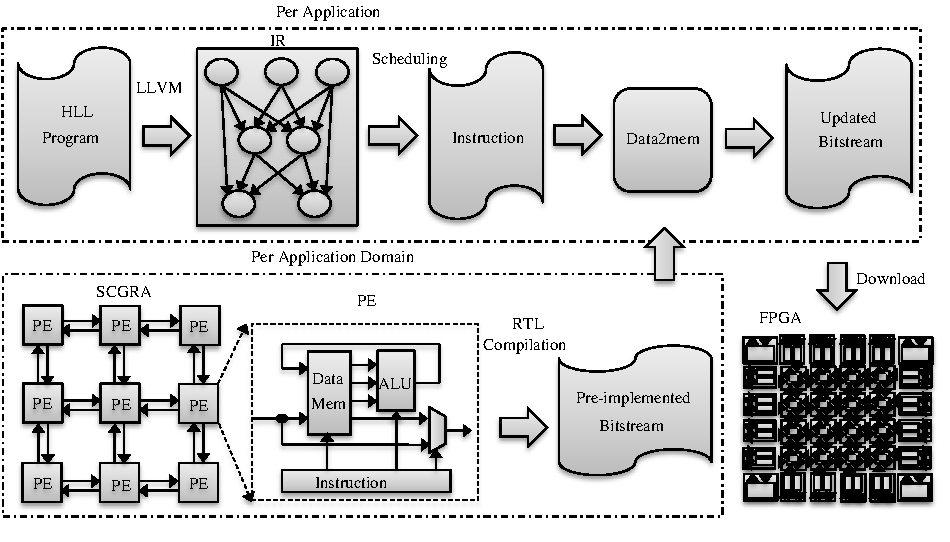
\includegraphics[width=10cm]{designflow}
\vspace{-1em}
\caption{Overview of the proposed soft coarse-grained reconfigurable array based high-level synthesis design methodology.}
\label{fig:design-methodology}
\vspace{-1em}
\end{figure*}

\section{Proposed Design Methodology}\label{sec:methodology}
%\subsection{A Two-Part Design Methodology}
\figref{fig:design-methodology} depicts an overview of the proposed high-level synthesis methodology.  As shown in the diagram, the proposed methodology can be divided into two distinct parts.  The first part, shown in the top half of the figure, is expected to execute frequently.  It should be executed every time a new design iteration is required, a new debug cycle is started, or simply when a new application within the same application domain is implemented.  On the other hand, the second part of the design flow, shown in the bottom half of the figure, is expected to execute infrequently, perhaps on a per-application domain basis.  Towards the end of the top half of the flow, the scheduling result is merged with the pre-built bitstream from the bottom half to produce the final downloadable bitstream for the target FPGA.

\subsection{Per Application Domain Steps}
The goal of the bottom half is to produce a highly optimized SCGRA for the target application domain.  The resulting SCGRA should capture key computational characteristics common to the target application domain.  For example, depending on the application domain, either fixed point number or floating number system may be employed.  The kinds of supported operations in the processing element (PE) may also be fine-tuned at this stage.  For instance, complex mathematical operations may be useful in one application domain while they may be omit to conserve hardware resources in other cases.  Finally, system-wide parameters, such as the number of PE employed, the PE connection topology, I/O bandwidth and data memory size should also be considered.

Note that since the design of the CGRA is soft, it is always possible to implement a different SCGRA as deemed appropriate.  Therefore, the design for the bottom half should be considered a best effort design.  It represents a tradeoff between generality and efficiency -- A generic solution helps to avoid executing the lengthy bottom half, saving compilation time, but will inadvertently consume more hardware resources, impacting the maximum clock frequency of the implementation.  In \secref{sec:scgra}, one class of such SCGRA suitable for our targeted benchmark application will be used to demonstrate how such array can been optimized to execute on extreme frequency of the target FPGA.

\subsection{Per Application Steps}
The goal of the top half of the design flow is to compile the specific user application to execute on the pre-compiled SCGRA.  Since no low-level FPGA implementation tool is involved, the runtime is comparable to common software compilation time of large systems.  This enables significant reduction in application development time so long as the SCGRA has already been implemented.  The reduced compilation time has net effect on increasing number of achievable debug cycles per day, greatly enhancing the productivity of the designers.

There are three sub-steps in the top half.  First, application developed in high-level languages are compiled into an intermediate representation (IR), which in our case, is the data flow graph (DFG) of the compute kernel.  Subsequently, a scheduler is invoked to schedule the DFG onto the SCGRA, taking into account the architectural features.  Finally, based on the scheduling results, the cycle-by-cycle control words for each PE within the SCGRA is generated and merged into the pre-built bitstream from the bottom half, producing the final updated bitstream for download.


%The per application layer targets at the implementation of a specific application. It abstracts IR from HLL program using LLVM \cite{llvm} first. Then it schedules the IR to a pre-implemented SCGRA using a delicate list scheduling algorithm. At the end of the scheduling, the control words that dictate all the activities of the SCGRA are dumped. (Since the control words are used to control the SCGRA cycle by cycle, we also call the control words instructions.) When all the instructions are collected, they are sent to the Xilinx tool data2mem \cite{data2mem} together with the pre-implemented bitstream. Thanks to this ISE independent tool, the instruction memory context of the pre-implmented SCGRA bitstream can be replaced with the new instructions directly and a new bitstream is generated. The new bitstream is actually an implementation of the application and can be downloaded to FPGA. Details of the design methodology will be elaborated in the following sections.


\subsubsection{Applications To IR}
The first step of our compilation process is to process the user application described in high-level languages into a common intermediate representation (IR) for the subsequent scheduling step.  In our current implementation, we have opted to make use of the open source LLVM compiler infrastructure \cite{llvm} for this task.  Apart from having a wide community support, one of the advantages of utilizing LLVM rests on its many readily available front-end for different languages such as C/C++, Java, .NET, Python, etc.  This allows easy extension of our work in the future across many different application domains.  Currently our applications are written in C.

Given an input application, we begin with manually identifying compute kernels that will be accelerated by FPGAs.  Once identified, the compute kernels undergo a series of reshaping to increase the amount of available parallelism.  For this purpose, we have initially opted to fully unroll the inner loops of the compute kernels.  We note that fully unrolling loops may not always be feasible and may not result in an optimal design.  This is left as future extension to this work while we focus on the overall design methodology here.


%The proposed HLS methodology mainly targets at accelerating the computation intensive kernels using FPGA. Typically the computation kernels can be loops with large iterations or functions called repeatedly and it is not applicable to deploy an extensively expanded kernel to FPGA due to the resource constrain and the IO constrain. Meanwhile, the primitive computation kernel body can be light weight and its parallelism is insufficient for FPGA acceleration. In this case, a computation kernel can be appropriately reshaped using techniques such as partial unrolling, such that the entire kernel can be divided into a number of identical kernel bodies and the computation kernel can be accelerated by simply deploying the kernel body to FPGA. When the kernel bodies are independent with each other, arbitrary number of kernel bodies can be put together and the reshaping is pretty simple. When the kernel bodies are dependent with each other, the reshaping problem gets complex. A preliminary solution to this problem is based on modulo scheduling \cite{rau1994iterative}. With modulo scheduling, the operations of the computation kernel can be pipelined. By ignoring the prologue part and epilogue part of the pipeline, the main part of the pipeline can be viewed as a group of identical computation bodies with different scales. Consequently, the computation kernel with dependent kernel bodies can also be reshaped as required. The reshaping scheme is not the focus of the paper and extensive efforts are still needed to figure out an optimal solution, sowe leave this for future study. In this paper, we assume that we are accelerating an computation kernel body. Also note that the term 'computation kernel body' is regarded as 'computation kernel' for the sake of convenience in the following sections. 

%The output DFG describes the data dependency of the HLL program, and helps explore operation parallelism during the SCGRA scheduling step especially for these computation kernels. Hence, it is considered as IR of our HLS methodology. 


The identified compute kernel is subsequently compiled to the machine-independent assembly language of LLVM through its Clang frontend for C/C++ programs.  It is then processed within the LLVM framework in preparation for intermediate DFG generation.  Several LLVM passes, including dead code elimination, loop simplification, and function inline are employed as optimization.  Moreover, branch instructions within the kernel body are merged into simple basic blocks by the introduction of PHI instructions.  Finally, once the code is transformed into static single assignment (SSA) style, it goes through our in-house pass that transforms the LLVM assemble code into a DFG ready for SCGRA scheduling. 

\subsubsection{SCGRA Scheduling}
In the SCGRA scheduling step, a list scheduling algorithm similar to \cite{colinheart} is adopted to schedule the DFG to the SCGRA infrastructure. It statically schedules the entire DFG on the target SCGRA. Such statically scheduled architecture is crucial in keeping the target SCGRA simple and efficient. To adapt to the proposed SCGRA structure, the scheduling metric is delicately adjusted to compromise the communication cost and load balance.

%The basic list scheduling process is relatively straightforward as shown in \algref{alg:sch}. Initially, it constructs an operation list in which all the operations have their source operands ready. Then it goes to the scheduling kernel. In the scheduling kernel, the PE that meets the PE selection metric is selected first. After that, the operation that fits the selected PE best according to the operation selection metric is chosen. As both the PE and the operation are determined, it gets to commit the scheduling, which includes finding the shortest routing paths, moving source operands to target PE along the routing paths and calculating the operation on target PE. Finally, it updates the operation list and repeats the scheduling kernel until the list becomes empty. In this work, we have made a few modifications on PE selection metric and operation selection metric to adapt to the DFG characteristics and the target SCGRA structure.

%\begin{algorithm}
%\caption{The SCGRA scheduling algorithm.}
%\label{alg:sch}
%\begin{algorithmic}
%\PROCEDURE{ListScheduling}
%\STATE Initialize the operation ready list $L$
%\WHILE {$L$ is not empty}
%\STATE select a PE $p$
%\STATE select an operation $l$
%\STATE OPScheduling($p$, $l$)
%\STATE Update $L$
%\ENDWHILE
%\ENDPROCEDURE
%
%\PROCEDURE {OPScheduling($p$,$l$)}
%\FORALL {predecessor operations $s$ of $l$}
%\STATE Find nearest PE $q$ that has a copy of operation $s$
%\STATE Find shortest routing path from PE $q$ to PE $p$
%\STATE Move operation $s$ from PE $q$ to PE $p$ along the routing path
%\ENDFOR
%\STATE Do operation $l$ on PE $p$
%\ENDPROCEDURE
%
%\end{algorithmic}
%\end{algorithm}

%Since each node of the DFG represents an operation and the DFG is actually a fine-granularity task graph, the PEs have much less time slots idle and can be busy all through the scheduling. In this case, we simply set the time interval that PE has been idle as the PE selection metric to find out the PE that guarantees the earliest computation. In addition, we also add PE utilization constrain to narrow down the PE candidates and help the scheduler to keep load balance. At the same time, we notice that the operation number of the DFG typically is much larger than the PE number of the SCGRA. There are sufficient ready operations in the DFG for scheduling and it makes little difference whether the operations on critical paths are executed earlier or later. As the routing cost between PEs is large due to the deep SCGRA pipeline depth and routing distance becomes essential to the scheduling performance, we set the routing cost that it takes the scheduler to move all the source operands to target PE as operation selection metric. Moreover, we also keep all the operand storing records, and each operand may have multiple copies across the CGRA. When an operand is needed for computation, we always fetch the source operand from the nearest PEs to further reduce the routing cost.

%In order to move a source operand to the selected PE, the scheduler must reserve all necessary hardware resources along the entire routing path for each corresponding time slot.  As the SCGRA status is changing through the scheduling process, a determined routing will soon deteriorates the scheduling performance. In this work, we take the time interval that it costs to move an operand from upstream PE data memory to downstream PE data memory as the link weight. Link weight is updated in real time and thus it indicates the routing congestion information of each link. With all the link weight across the SCGRA updated, we further calculate the routing path of a PE pair using Dijkstra algorithm. Since the Dijkstra algorithm here takes both the routing distance and routing congestion information into account, it helps to find out a near optimal routing in real time and is able to provide a fast operation transmission.

%On top of the issues mentioned, the scheduler is also responsible for the data memory management. The data memory management mainly involves two aspects. On the one side, it slightly adjusts the operation selection to reduce the intermediate operands that need to be stored in data memory and to make sure that the data memory does not overflow. In this work, we add an operation selection filter, which removes the operations with larger children operations from operation ready list, to control the data memory requirements. Note that this scheme is not able to precisely adapt the data memory consumption and it also influences the scheduling performance. Fortunately, the experiments show that the primitive data memory capacity is sufficient to fulfill the requirements of the computation kernels even without stringent filtering. 

%On the other side, the data memory manager also needs to generate read/write addresses that will become part of the instructions. Since the data memory requirements are not pressing, a static address generation is adopted. It does not start until the scheduling kernel is completed, so both an operand's read time $\left( tr_1, tr_2,...,tr_m \right)$ and write time $\left( tw_1,tw_2,...,tw_n \right)$ on a data memory can be obtained from scheduling records. Note that $tr_1<tr_2<...<tr_m$ and $tw_1<tw_2<...<tw_n$. In most occasions, $n=1$, but $n \geq 1$ sometimes because the routing path is changing all the time. An address is allocated to the operand at the first time it is stored in the data memory and the address is released at the last time it is referenced through the data memory. Therefore, the lifetime of the operand in the data memory is from $tw_1$ to $tr_m$.

%Upon completion of the scheduling stage, a cycle-accurate schedule of the operation on each PE, as well as the movement of data between the data memory and the PEs in the SCGRA is obtained.  This schedule must then be encoded accordingly and incorporated into the instruction ROM of the SCGRA.

\subsubsection{Bitstream Integration}
The final step in our proposed HSL methodology is to incorporate the instruction for each PE obtained from the scheduling stage with the pre-compiled SCGRA design.  By design, our SCGRA do not have mechanism to load in instruction streams from external memory.  Instead, we take advantage of the reconfigurability of SRAM based FPGAs and stored the cycle-by-cycle configuration words using on-chip ROM.  The content of these instruction ROMs are embedded in the configuration bitstream.  In particular, the organization of the instruction ROM in the place-and-routed SCGRA design is obtained from its XDL file \cite{beckhoff2011xilinx}, which in turn allows us to create the corresponding BMM file.  With this BMM file, the encoded instructions collected from the DFG scheduling may then be incorporated into the pre-implemented bitstream using the data2mem tool from Xilinx \cite{data2mem}.  
While original SCGRA design needs hours to implement, the bitstream updating scheme only costs a few seconds.




%\section{SCGRA Design} 
One key idea of the proposed design methodology is to rely on an intermediate SCGRA layer to improve compilation time of the high-level user application.  While the exact design of this SCGRA does not affect the compilation methodology, its implementation does have a significant impact on the performance of the generated gateware.  
In this section, an instance of such SCGRA design is thus presented to demonstrate the feasibility of producing high performance gateware without incurring long compilation time.  As shown in \figref{fig:pe}, the PE of this SCGRA is highly optimized for FPGA implementation, centering its design around a hard DSP block with the addition of an instruction ROM and a multi-port data memory.  In addition, a load/store path is implemented on the PEs that are responsible for data I/O beyond the FPGA.
Using this design as a template, it is envisioned that a separate hardware design team, or the high-level compiler may be able to produce similarly high-performance SCGRA that is optimized for the targeted application domain.

%The SCGRA serves as the hardware infrastructure of the proposed HLS methodology. On one hand, it should be more flexible than traditional CGRA, so that it can meet different requirements by customizing a few sub components of the SCGRA and keep the hardware overhead small. On the other hand, it should be more general than FPGA, so that it allows us to reuse the low level optimizations such as data path pipelining and improve design productivity as well. With the two design goals in mind, a 2D Torus SCGRA template is developed. It is composed of homogeneous PEs, so we can simply focus on the PE structure. The PE structure is shown in Figure \ref{fig:pe}. It basically consists of an ALU, a ROM based instruction memory and a multiple-port data memory. To connect with the system out of the FPGA, load/store data path is added to the PEs with IO interface. Details of the PE components are illustrated in the following sections.

\label{sec:scgra}
\begin{figure}[h]
\centering
\includegraphics[width=7cm]{pe}
\vspace{-1em}
\caption{PE structure}
\label{fig:pe}
\vspace{-1em}
\end{figure}

\subsection{Instruction Memory and Data Memory}
There are two types of memory in each PE.
The instruction memory stores all the control words of the PE in each cycle.  Since its content does not change during runtime, a ROM is used to implement this instruction memory.  The content of the ROM is loaded together with the configuration bitstream.

%When the instruction memory can be implemented using a single primitive BRAM, it is able to work at extreme frequency of the FPGA device. However, the timing gets pressing when the instruction memory becomes larger. In order to improve the timing of instruction memory, the Fixed Primitives scheme is adopted when we construct the instruction memory using core generator. Meanwhile, as a single instruction is distributed to multiple primitive BRAMs, it will be better to put control bits going to the same sub components of PE such as DSP48 to the same primitive BRAM accordingly. This strategy makes the placing and routing easier and hence improves the timing. In addition, registers can be added to the output port of the instruction memory to pipeline the critical paths originated from the instruction memory.

On the other hand, data memory stores intermediate data that can either be forwarded to the PE downstream or be sent to the ALU for calculation.  For fully parallelized operation, \emph{at least} four read ports are needed -- three for the ALU and one for data forwarding.  Similarly, at least two write ports are needed to store input data from upstream memory and to store the result of the ALU in the same cycle.
Although a pair of true dual port memories may seems to be able to satisfy this port requirement, conflicts may arise if the ALU needs to read the data while the data path needs to be written.  As a result, a third dual port memory is replicated in the data memory.


%Since BRAM in Xilinx FPGA initially has read ports and write ports shared, a duplicated true dual port memory is able to satisfy the requirement. However, there will be no write port available when ALU reads data for calculation, which can't meet the needs of fully pipelined ALU. In this case, maximum ALU throughput is cut down to be 0.5. To avoid this bottleneck, we duplicate another true dual port BRAM in the data memory. Three read ports are allocated to ALU and the rest are used for forwarding.

%\begin{figure}
%\centering
%\subfloat[Two write ports and four read ports] {\label{fig:w2r4} 
%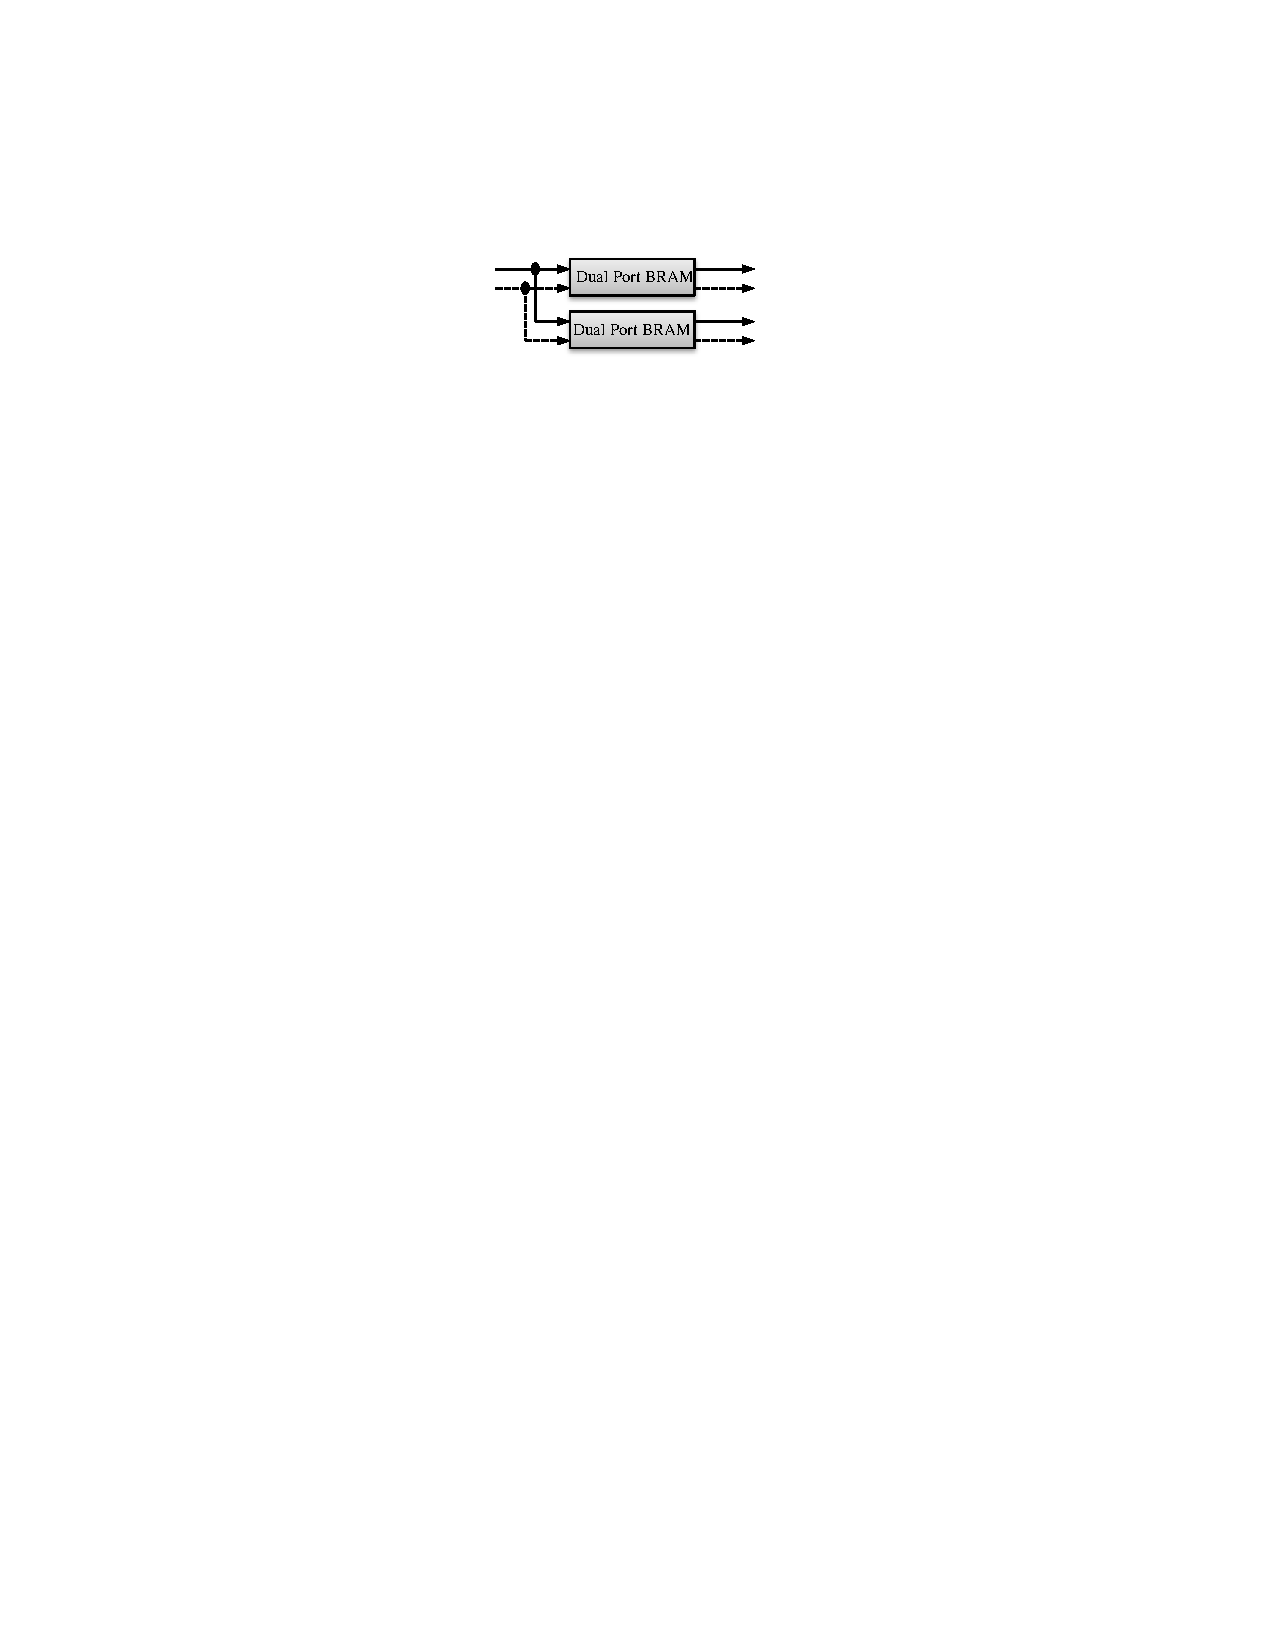
\includegraphics[width=4cm]{w2r4}}\\
%\subfloat[Three write ports and six read ports] {\label{fig:w3r6} 
%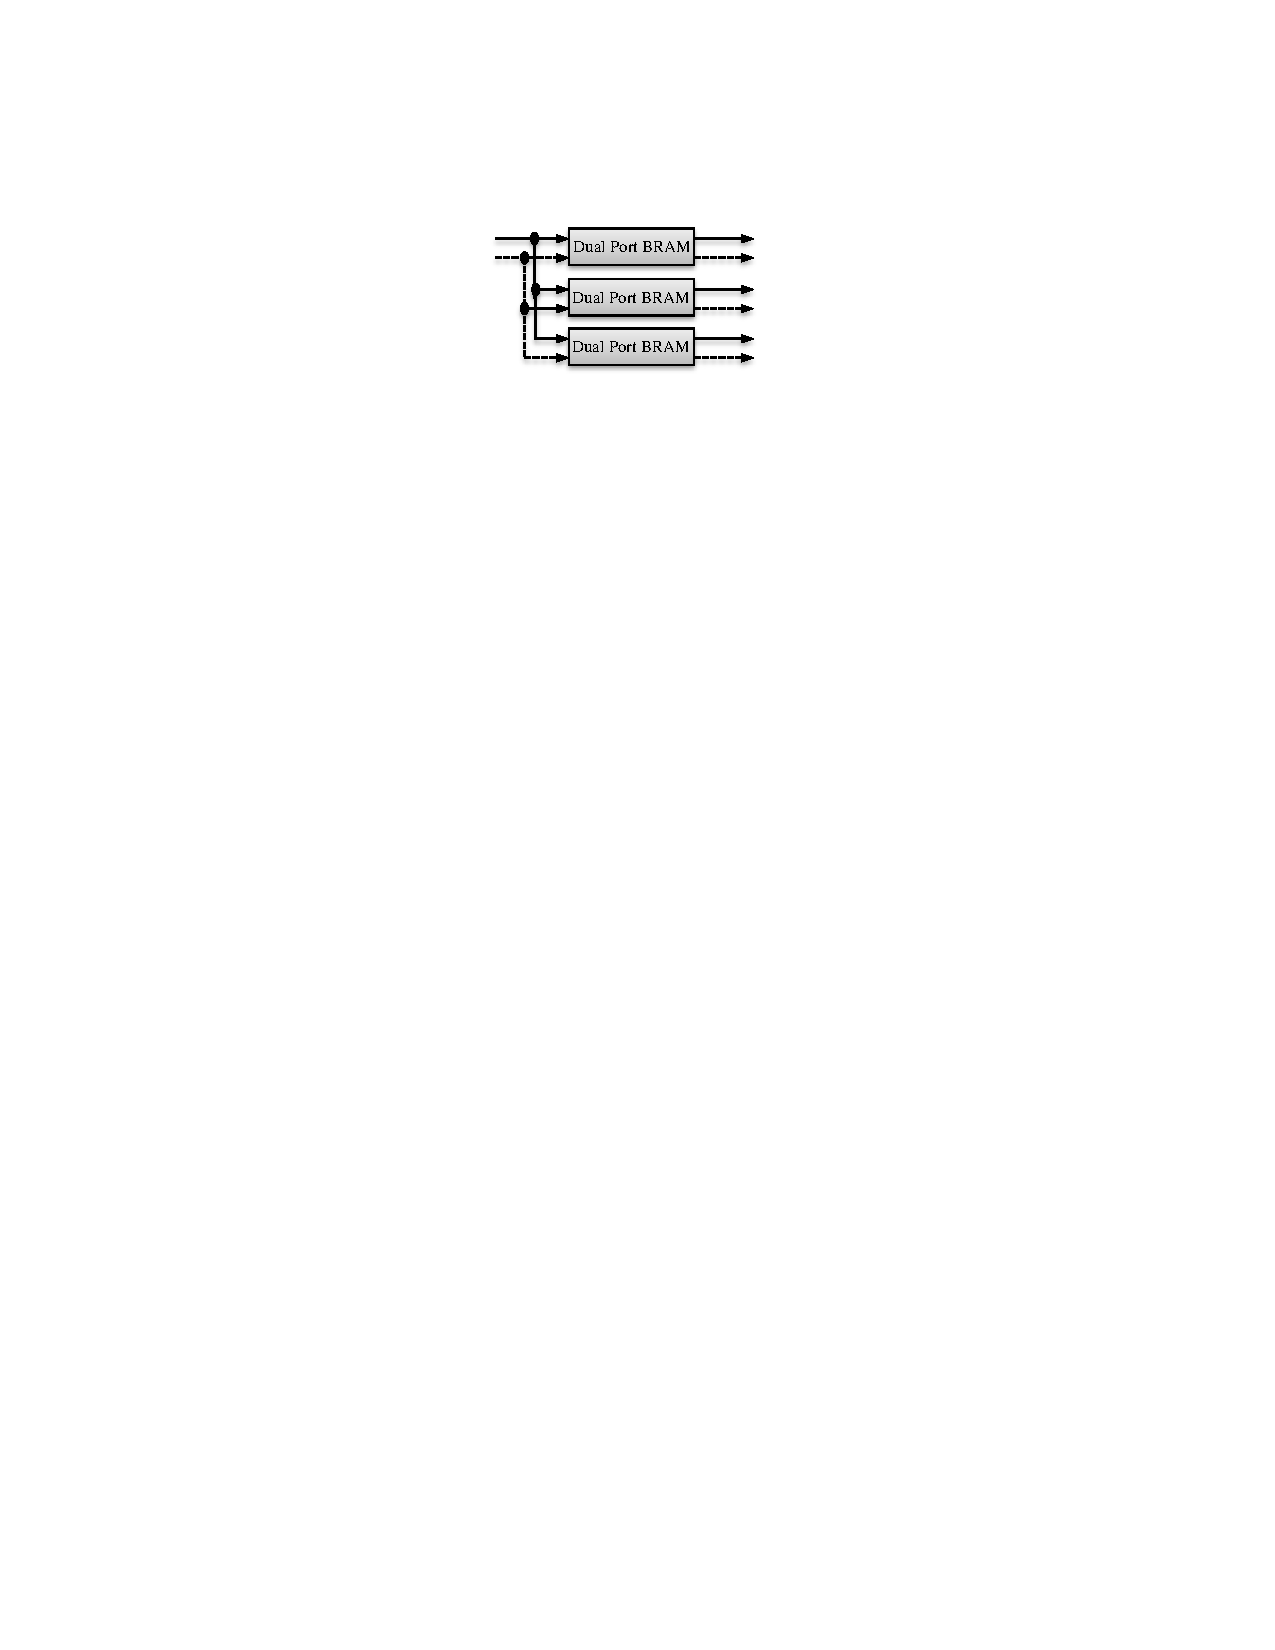
\includegraphics[width=4cm]{w3r6}}
%\caption{Multiple-port data memory}
%\label{fig:datamemory}
%\end{figure}

\subsection{ALU}
At the heart of the proposed PE is an ALU designed around the DSP core in the target Xilinx FPGA as shown in \figref{fig:ALU}.  The DSP core is responsible for all basic arithmetic operations such as multiply-add.  In addition, operations that are not provided by the DSP blocks such as add, sub and xor are handled by the 3-stage pipeline that takes the form of  $in1$ <$OP1$> $in2$ <$OP2$> $in3$.  Finally, a special PHI operation was embedded in the template to handle the applications that have branches merged. The PHI operation was implemented simply as a multiplexer, which has little influence on the final PE timing. 

%Since the proposed HLS methodology targets at computation intensive application kernels, the operations needed are basically arithmetic operations and logic operations. 
%Figure \ref{fig:ALU} shows a three-stage pipeline ALU template which is able to cover these operations. 
%DSP core in Xilinx FPGA, which has already included quite a few operations such as multiply-add, is widely used in computation applications and it is able to operate at extreme speed configured with three-stage pipeline, so we integrate it in the ALU. For the operations that are not covered, a three-stage template $in1$ <$OP1$> $in2$ <$OP2$> $in3$ is developed. $OP1$ and $OP2$ can be any operations that fit in single-stage pipeline. When $OP1$ and $OP2$ are replaced with the operations such as add, sub, and xor, the template is also able to work at full speed. In addition, we also have a special PHI operation embedded in the template to handle the applications that have branches merged. PHI operation is actually a multiplexer, so it has no influence on the timing. 

\begin{figure}
\centering
\includegraphics[width=6cm]{alu}
\vspace{-1em}
\caption{ALU Template}
\label{fig:ALU}
\vspace{-1em}
\end{figure} 

\subsection{Load/Store Interface}
For the PEs that also serve as I/O interface to the SCGRA, an additional load/store path is implemented.  In this work, the input data are assumed to be available in the scheduled order via an input FIFO.  As such, only one additional signal bit is needed to control the popping of the FIFO.   Similarly, another single bit signal is used to decide whether data should be pushed into the output FIFO.  These control bits are similarly stored using the reserved bits in the proposed instruction format.


% Since there are still reserved bits left in instruction memory, the control bits simply stored in instruction memory. Note that load path results in larger multiplexer, and additional pipeline register is added to solve this problem.

%\section{Experiments}\label{sec:results}
In this section, we take 5 computation kernels including matrix multiply (MM), fast Fourier transform (FFT), discrete convolution (CONV), advanced encryption standard (AES) and Viterbi decoder (VD) as our benchmark. The benchmark is implemented using the proposed HLS methodology and a direct mapping methodology respectively. After that, compilation time, hardware implementation efficiency and performance of the two distinct design methodologies are compared.

\subsection{Benchmark}
MM has two input matrices and an output matrix. In the experiment, we set the matrix dimension to be $20 \times 20$. And there are 8000 multiply-add operations.

FFT initially takes complex vector $x \left( i \right)$ as input, and complex vector $X \left( i \right)$ as output where $i=1,2,3,...,N,N=2^M, M \in \mathbb{Z}$. In order to escape Sine and Cosine computation on FPGA, roots of unity vector are also considered to be input data. In the experiment, we set $N=256,M=8$ and all the complex operations are further transformed to real operations. Finally, there are 8192 real multiply-add operations.

Input signal vectors of CONV are $u \left( i \right)$ and $h \left( i \right)$ where $i=1,2,3,...,N$. The output signal vector can be expressed as follow: \begin{displaymath} y \left( k \right) = \sum_{i=1}^N {u \left( i \right) \times h \left( k-i \right),k=N/2,N/2+1,...,3N/2} \end{displaymath} In the experiment, $N=100$ and there are around $3N^2/4$ multiply-add operations.

AES adopts 128-bit key and takes 7 128-bit blocks as input. There are 8864 operations mainly including circular shift and bitwise exclusive or.

VD adopts the NASA standard in which the decoding rate is $1/2$ and the decoding length is 7. Input message length is 150 bit and the total operation number is around 2989 including shift, add, or and compare.

\subsection{Experiment Setup}
All runtimes were obtained on a Linux workstation with an Intel(R) Xeon(R) CPU E5345 and 8GB of RAM. All the implementations targeted Xilinx Virtex6 FPGA (xc6vlx240tff784-1). The proposed HLS methodology employed LLVM v3.2 and clang v3.2 for C program compiling and PlanAhead v13.4 for the SCGRA implementations. As for the direct mapping methodology, \autoesl 2011.4.2 was taken as a representative. Additionally, both design methodologies provided three implementations with different trade-off between performance and hardware overhead for a comprehensive comparison.

\autoesl achieves the trade-off between hardware overhead and performance mostly through altering the loop unrolling factor. Three sets of implementations including no unrolling, medium unrolling and large unrolling were experimented. Configurations of the unrolling for each benchmark are summarized in \tabref{tab:urconfig}. Also, note that all the implementations were set to be fully pipelined using \autoesl directive. In addition, we assumed that the FPGA had direct shared access to the main system memory with the CPU and only a single memory port was presented. As \autoesl transforms each input/output array/vector to a separate input/output memory port, all the input/output arrays/vectors were reorganized as a single input/output vector to ensure that the implementations meet the IO requirement. 
 
\begin{table}[h]
\vspace{-1em}
\caption{Detailed unrolling configurations of the benchmark}
\label{tab:urconfig}
\centering
\small
\begin{tabular}{|p{1cm}|p{6.5cm}|}
\hline
MM & {It is a three-level nested loop and each loop iterates 20. Unrolling factors of three implementations are  $1 \times 1 \times 1$, $1 \times 5 \times 20$ and $1 \times 10 \times 20$.
}\\

\hline
FFT & {It is a three-level nested loop. The outmost loop iteration number is 8 while the iteration number of the rest two loops varies with the outmost loop. Unrolling configurations of the three implementations are $1 \times 1 \times 1$, $8 \times 1 \times 1$ and $8 \times m \times n$, $m \times n$ is fixed to be 32. 
%\autoesl fails to complete the implementation when I further increase the unrolling factors.
}\\

\hline
CONV & {It is a two-level nested loop and each loop iterates 100. Unrolling configurations of the three implementations are $1 \times 1$, $1 \times 100$, $5 \times 100$.}\\

\hline
AES & {AES kernel procedure iterates 9. Unrolling configurations of the three implementations are 1, 3, and 9.
%I tried to unroll and inline the sub functions manually, \autoesl failed to implement the design.
}\\

\hline
VD & {VD kernel iterates 150. Unrolling configurations of the three implementations are 1, 2 and 5.}\\

\hline
\end{tabular}
\vspace{-1em}
\end{table}

The proposed HLS methodology obtains the trade-off between hardware overhead and performance by altering the number of PEs in the SCGRA. Three SCGRA designs, with the PEs connected as a $4 \times 4$ Torus, a $3 \times 3$ Torus and a $2 \times 2$ Torus were developed. Each PE contained a $256 \times 16$-bit data memory. The ALU within each PE supported 8 types of operations and thus required a 3-bit opcode.
In total, PEs without I/O port required 65-bit instruction and PE with I/O required one additional bit for load/store FIFO operations. Since the size of a primitive BRAM on the device was 18K-bit or 36K-bit, we built instruction ROMs with 72-bit width. Furthermore, to cater for different benchmark sizes, 7 instruction ROM sizes -- 1K$\times$72-bit, 2K$\times$72-bit, 4K$\times$72-bit, 6K$\times$72-bit, 8K$\times$72-bit, 10K$\times$72-bit and 12K$\times$72-bit -- were considered. Combining with the 3 different SCGRA sizes, a total of 21 different SCGRA designs were implemented as target SCGRA platforms.

\subsection{Experiment Results}
In this section, comparisons of compilation time, hardware implementation efficiency and performance using both design methodologies are presented in detail. 
%However, the proposed HLS methodology depends on a pre-build SCGRA. While we have only 9 SCGRA implementations in advance at the moment, not all the computation kernels in the benchmark are able to find a matched pre-build SCGRA. When the benchmark fails to find any pre-build SCGRA, we consider it as an implementation failure. 
%In particular, FFT and AES failed to be implemented on the pre-built 2$\times$2 Torus SCGRA, while VD failed to be deployed to any of the pre-built SCGRA.
%In these cases, the implementation results are left blank in the figures. 

\subsubsection{Compilation Time}
Given a HLL program, the HLS tools should be responsible for the entire process transforming the program all the way to bitstream. Therefore the compilation time that the process consumes is considered to be the metric of the design tools' efficiency. 

Figure \ref{fig:designtime} shows the compilation time of the benchmark using both \autoesl and the proposed HLS methodology. \autoesl includes two steps: \autoesl synthesis and \autoesl implementation. Generally speaking, the time spent on \autoesl synthesis is relatively short, ranging from seconds to dozens of seconds. However, the resulting design must go through the lengthy back-end implementation tools such as floor planning, mapping and placing-and-routing. As a result, the compilation time of a single computation kernel with moderate loop unrolling costs around 20 minutes. Larger loop unrolling that requires more hardware components further slows down the \autoesl implementation process. As shown in the Figure \ref{fig:designtime}, the compilation time of FFT and VD with large loop unrolling even exceeds 2 hours.

\begin{figure}[h]
\centering
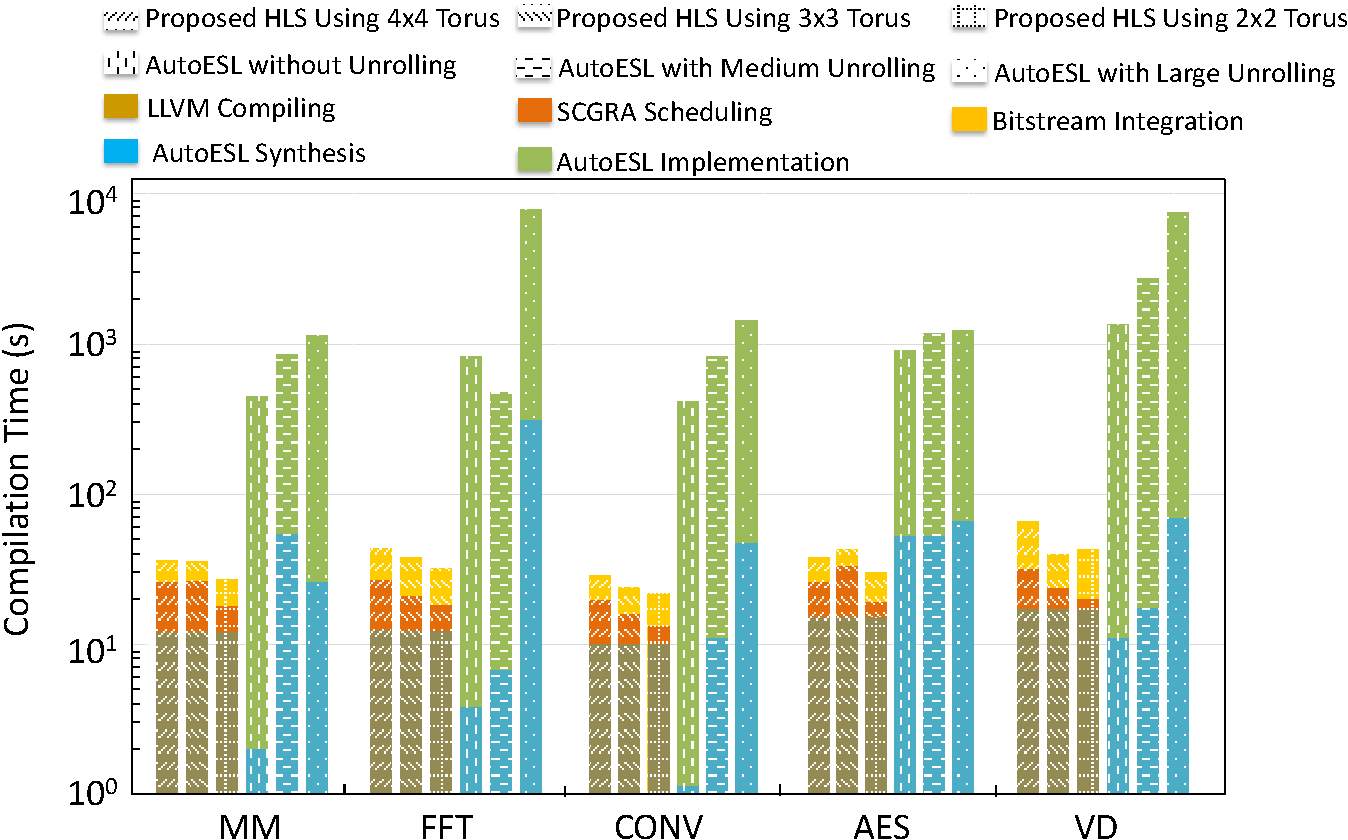
\includegraphics[width=8cm]{designtime}
\vspace{-1em}
\caption{Compilation time comparison of the benchmark using both \autoesl and the proposed HLS methodology}
\label{fig:designtime}
\vspace{-1em}
\end{figure} 

On the other hand, the proposed HLS methodology bypasses the lengthy low-level implementation steps and simply needs three high-level steps: LLVM compiling, SCGRA scheduling and bitstream integration. Each of these steps could be completed in a few seconds and implementation using this methodology is generally 10X-100X faster than even the smallest implementation using \autoesl.

\subsubsection{Hardware Implementation Efficiency}
In this section, hardware implementation including both hardware resource overhead and implementation frequency using the two design methodologies are compared.

Table \ref{tab:overhead} presents the hardware overhead of the benchmark using the proposed HLS methodology with $4 \times4$ Torus(P44), $3 \times 3$ Torus (P33), and $2 \times 2$ Torus (P22), and \autoesl with no unrolling (NUR), medium unrolling (MUR), and large unrolling (LUR). From the table, it can be seen that the proposed HLS methodology tends to use more BRAM than \autoesl does in all the occasions. The prime reason is that the proposed HLS methodology employs SCGRA as the hardware infrastructure and the SCGRA typically requires a number of large instruction memories to store all the control words (instructions). Actually, the BRAM consumption using the proposed HLS methodology roughly equals to the SCGRA scale multiplied by the scheduling result of the target application. It is also the resource bottleneck of the proposed HLS methodology. Hopefully, the context compression techniques \cite{kim2010dynamic} used in CGRA design may help remove the instruction redundancy and alleviate the BRAM requirements. While \autoesl mainly uses BRAM for buffering between different sub blocks and IO, the BRAM requirement is much lower because there are few sub blocks in the benchmark. 

\begin{table}[h]
\vspace{-1em}
\caption{Hardware overhead of the benchmark.}
\label{tab:overhead}
\centering
\small
\begin{tabular}{|c|c|c|c|c|c|c|}
\hline
\multicolumn{2}{|c|}{} & SLICE & LUT & FF & DSP & RAM\\
\hline
\multirow{4}{*}{MM} & T44 & 2273 & 4303 & 11129 & 16 & 176\\
\cline{2-7}
& T33 & 1029 & 3229 & 6958 & 9 & 99\\
\cline{2-7}
& T22 & 619 & 1045 & 2805 & 4 & 76\\
\cline{2-7}
& NUR & 158 & 296 & 320 & 1 & 2\\
\cline{2-7}
& MUR & 1151 & 3517 & 4224 & 78 & 2\\
\cline{2-7}
& LUR & 1958 & 6711 & 8006 & 182 &2\\
\hline

\multirow{4}{*}{FFT} & T44 & 2273 & 4303 & 11129 & 16 & 176\\
\cline{2-7}
& T33 & 1519 & 2574 & 6976 & 9 & 171\\
\cline{2-7}
& T22 & 619 & 1045 & 2805 & 4 & 76\\
\cline{2-7}

& NUR & 286 & 648 & 823 & 5 & 6\\
\cline{2-7}
& MUR & 595 & 1901 & 2024 & 32 & 20\\
\cline{2-7}
& LUR &	17190 &	49099 &	37283 &	654 & 20\\
\hline

\multirow{4}{*}{CONV} & T44 & 2273 & 4303 & 11129 & 16 & 176\\
\cline{2-7}
& T33 & 1029 & 3229 & 6958 & 9 & 99\\
\cline{2-7}
& T22 & 619 & 1045 & 2805 & 4 & 76\\
\cline{2-7}

& NUR &	87 & 217 & 205 & 1 & 2\\
\cline{2-7}
& MUR & 1149 & 3763 & 4558 & 98 & 2\\
\cline{2-7}
& LUR & 4213 & 13633 & 19940 & 497 & 2\\
\hline

\multirow{4}{*}{AES} & T44 & 2273 & 4303 & 11129 & 16 & 176\\
\cline{2-7}
& T33 & 1029 & 3229 & 6958 & 9 & 99\\
\cline{2-7}
& T22 & 620 & 1395 & 2817 & 4 & 108\\
\cline{2-7}

& NUR &	501 & 1251 & 1660 & 0 & 8\\
\cline{2-7}
& MUR &	705 & 1799 & 1947 & 0 &	8\\
\cline{2-7}
& LUR & 708 & 1767 & 1872 & 0 & 8\\
\hline

\multirow{4}{*}{VD} & T44 & 2782 & 4811 & 11209 & 16 & 806\\
\cline{2-7}
& T33 & 1668 & 2544 & 6325 & 9 & 387\\
\cline{2-7}
& T22 & 725 & 1298 & 2825 & 4 & 172\\
\cline{2-7}

& NUR & 1911 & 4883 & 6684 & 0 & 12\\
\cline{2-7}
& MUR & 3306 & 10033 & 12863 & 0 & 12\\
\cline{2-7}
& LUR & 8833 & 24693 & 31886 & 0 & 12\\
\hline
\end{tabular}
\vspace{-1em}
\end{table}

As for SLICE, LUT, FF and DSP, the consumption using the proposed HLS methodology mainly depends on the SCGRA scale, and it fluctuates within a narrow range when the instruction memory capacity varies. While the consumption of these components using \autoesl increases dramatically with the loop unrolling factor and it will soon eat up all the FPGA resource. When the computation kernels are not unrolled at all, \autoesl provides quite compact implementations and it consumes only a small number of SLICE, LUT, FF and DSP. When the medium loop unrolling is adopted, \autoesl and the proposed HLS methodology cost comparable number of the primitive components. When a large loop unrolling is employed, the overhead of these components using \autoesl turns to be larger than that using the proposed HLS methodology for most applications in the benchmark. The overhead comparison of AES is a bit different, because the SCGRA has more computation capability than that is required. Pre-built more light-weight SCGRA will decrease the SCGRA overhead.

Figure \ref{fig:impl_freq} shows the implementation frequency using both tools. It is clear that the SCGRAs employed in the proposed HLS methodology for all the kernels except VD are generally able to work around 400 MHz, which is close to the extreme frequency of the three-stage-pipelined DSP core implemented on the target FPGA. \autoesl has specific implementation for each benchmark, but the highest implementation frequency is only around 300MHz. When large loop unrolling is adopted, the implementation frequency deteriorates radically. The worst implementation frequency as presented in Figure \ref{fig:impl_freq} is only around 50 MHz, which offsets the performance improvement brought by the loop unrolling. Essentially, a large number of irregular blocks that randomly scatter around the FPGA using \autoesl increase the difficulty for place-and-route, causing a reduced implementation frequency. In contrast, the SCGRA is regular and well pipelined, therefore the implementation frequency is much higher. Figure \ref{fig:lib_impl_freq} displays the frequency of all the 21 SCGRA implementations. It demonstrates that the implementation frequency degrades gracefully with the increase of the SCGRA scale and instruction memory. 

\begin{figure}[h]
\centering
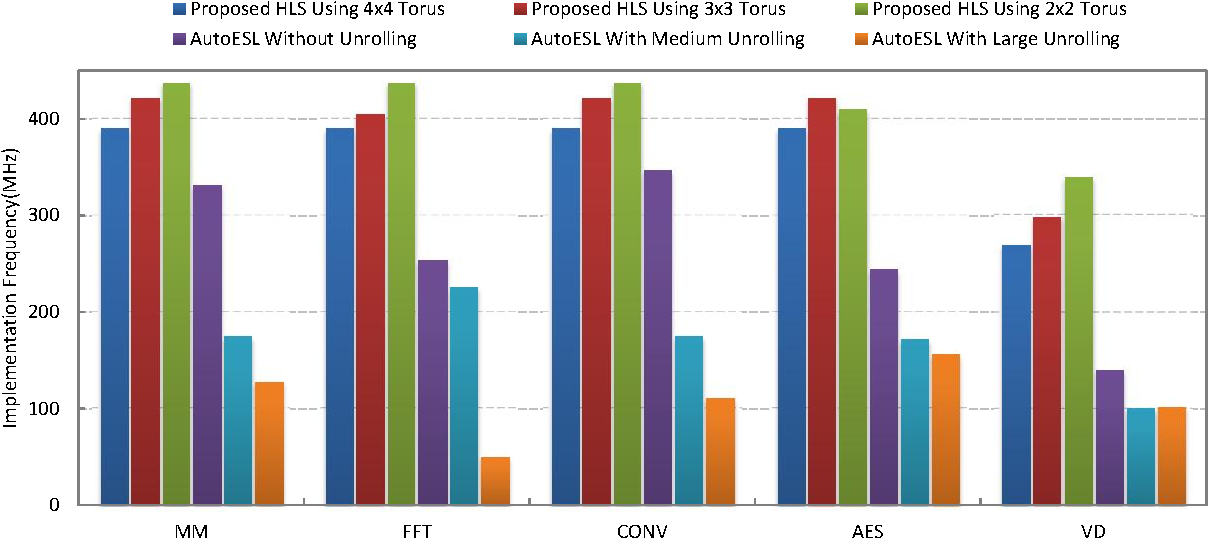
\includegraphics[width=8cm]{impl_freq}
\vspace{-1em}
\caption{Implementation frequency comparison of the benchmark using both \autoesl and the proposed HLS methodology}
\label{fig:impl_freq}
\vspace{-1em}
\end{figure}

\begin{figure}[h]
\centering
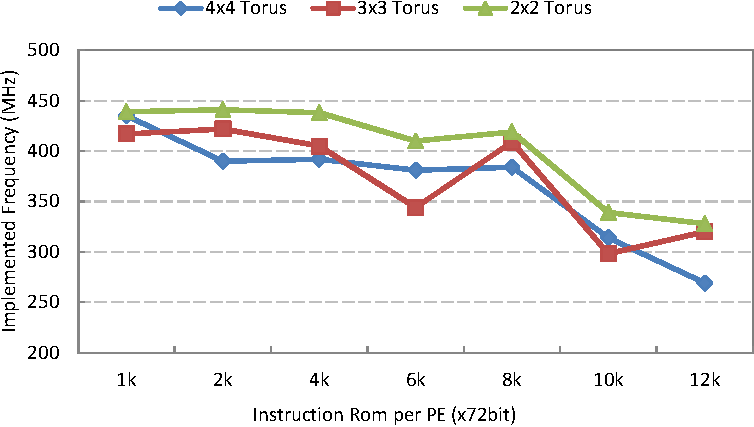
\includegraphics[width=6cm]{lib_impl_freq}
\vspace{-1em}
\caption{Implementation frequency of all the 21 SCGRAs}
\label{fig:lib_impl_freq}
\vspace{-1em}
\end{figure}


\subsubsection{Performance}
In this section, the execution time of the benchmark is taken as the metric of performance. The execution time is computed by multiplying the number of execution cycles with the implemented clock period. The number of execution cycles for \autoesl was obtained from the synthesis tools, while that of the proposed HLS methodology was obtained from the SCGRA scheduler. All clock periods of the implementations were obtained from timing reports of the final FPGA implementations.

Figure \ref{fig:sim_perf} presents the simulation performance (execution cycles) of the benchmark using both \autoesl and the proposed HLS methodology. Generally, larger loop unrolling using \autoesl leads to better simulation performance. Nevertheless, the performance gain brought by loop unrolling varies in a wide range. CONV with large loop unrolling is almost 20X faster than that without loop unrolling while AES barely benefits from the loop unrolling. The situations of MM, FFT and VD lie between the previous two extreme examples. Basically, there are three reasons for this:


First of all, single input port and single output port constrain the IO bandwidth, and potential parallel operations may be forced to be serial. This is part of the reason for all the unsatisfying performance acceleration. 

Second, \autoesl leaves the user to decide the loop unrolling. However, the design space can be extremely large and it is difficult for the user to decide the optimal unrolling factors especially under IO constrain. Take AES as an example. It consists of quite a few sub loops and \autoesl fails to unroll all the sub loops, so we have to leave some of the sub loops unchanged. These serial loops limit not only its own's execution time but also the unrolled loops in the downstream. In this case, randomly unrolling some of the sub loops may have little influence on the performance of the entire application. 

Third, source code structure may not be appropriate for \autoesl to synthesize. Take FFT as an example. FFT is a three-level nested loop, and the inner loops depend on the outmost loop. In fact, this is the reason that \autoesl fails to estimate the simulation performance. When the medium loop unrolling is adopted, we manually unroll the outmost loop into 8 stages. And it is natural to connect the 8 stage in serial manner according to the FFT structure. As each stage depends on one after another, the performance acceleration mainly relies on the overlapped computation across the stages. When the large loop unrolling scheme is employed, each stage is further unrolled. Since the neighboring stages communicate through RAM buffers which have limited IO ports, each stage still suffers the same communication bandwidth constrain and loop unrolling in a single stage is almost useless. Declaring multiple smaller vectors to guide \autoesl to synthesize more RAM buffers for communication between neighboring stages and delicately allocating the intermediate data to proper sub vectors to fully reuse the increased communication bandwidth may remove the inner communication bottleneck. Nevertheless, it is challenging for the user to reorganize the source code to fulfill such harsh requirements. In this experiment, two vectors are used to store real part and imaginary part of a complex intermediate data respectively between the neighboring stages. Therefore, it is not surprising that \autoesl fails to accelerate FFT much through the straightforward loop unrolling. 

As for the proposed HLS methodology, the performance is more predictable. According to Figure \ref{fig:sim_perf}, larger SCGRAs with more PEs generally provide higher performance and require more instruction memory while smaller SCGRAs are exactly the opposite. The only exception is VD and there are combined reasons for this. The SCGRA scheduler tends to keep load balance for better performance and operations are scattered across the SCGRA, but the parallel operations in VD are insufficient for scheduling and the communication gets more frequent. While communication in larger SCGRAs is more costly and the deep pipeline of the SCGRA makes the situation even worse, therefore, the smaller SCGRAs achieve even better performance than the larger SCGRAs. This problem can be alleviated by adjusting the scheduling strategy through slightly de-emphasizing the load balance.

\begin{figure}[h]
\centering
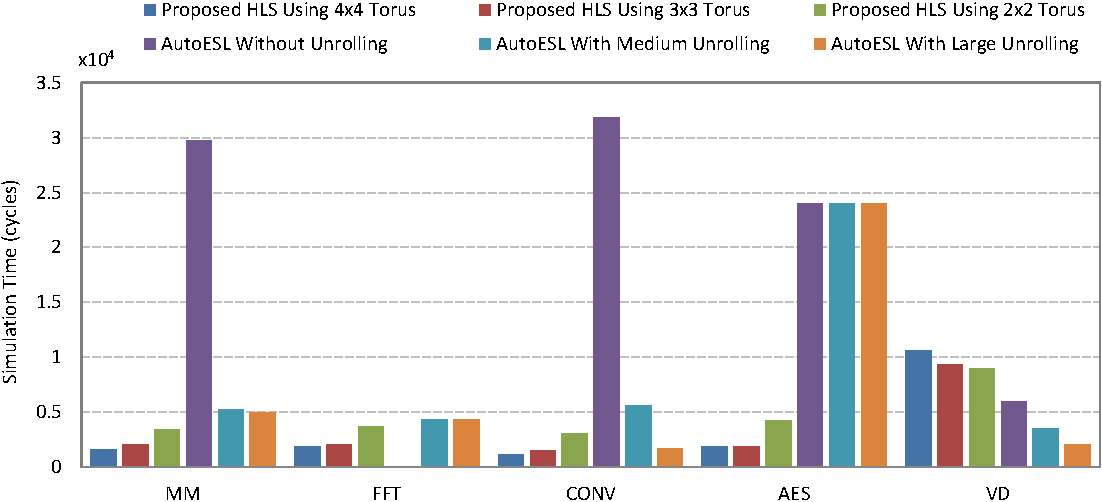
\includegraphics[width=8cm]{sim_perf}
\vspace{-1em}
\caption{Simulation performance comparison of the benchmark using both \autoesl and the proposed HLS methodology}
\label{fig:sim_perf}
\vspace{-1em}
\end{figure}

With the above analysis, we can conclude that the proposed HLS methodology outperforms \autoesl in implementing the benchmark with larger parallel computation but it is not quite effective in handling the benchmark with limited parallelism. Note that we are not denying that \autoesl is able to achieve optimal performance acceleration on FPGA. It is just difficult for the user to figure out proper source code structure and unrolling configuration for the optimal performance acceleration over such a broad design space. The proposed HLS methodology that builds SCGRA over FPGA actually scales down the design space. Meanwhile, the loops are fully unrolled and all the data dependency are completely exposed to the scheduler, so it is getting easier to find an near optimal solution. Particularly, the user simply needs to provide the SCGRA scale and maximum instruction memory depth and doesn't need to make any low level optimization decisions, which makes the design methodology more friendly to the user. 

With both the implementation frequency in Figure \ref{fig:impl_freq} and simulation performance in Figure \ref{fig:sim_perf}, the real performance of the benchmark using different HLS tools is acquired as shown in Figure \ref{fig:real_perf}. It can be seen that the proposed HLS method outperforms \autoesl in all the benchmark except VD. The highest performance of MM, FFT, CONV and AES using the proposed HLS method is around 7X, 4X, 5X and 21X faster than that using \autoesl respectively, while the performance of VD is a bit slower due to the limited parallelism and the performance acceleration is around 0.8X.

%On the other hand, the \autoesl implementations adopted RAM buffers as communication interfaces between blocks, which was incapable to provide enough bandwidth to support large parallelism exploration. Take the experiments of FFT and AES as an example. Both computation kernels of FFT and AES were divided into multiple sub-blocks to provide larger parallelism for \autoesl implementation. However, the dependent sub-blocks have to fetch data from RAM buffer in upstream and send data to RAM buffer in downstream. As a result, each sub block has additional I/O bandwidth constrains which negatively affected parallel execution. As a result, designs with larger unrolling factors failed to delivered the expected performance improvement. At the same time, the design with larger unrolling requires larger hardware resource and deteriorates the low-level implementation timing. Consequently, this has led to the performance degradation of FFT and AES with larger unrolling factors.

\begin{figure}[h]
\centering
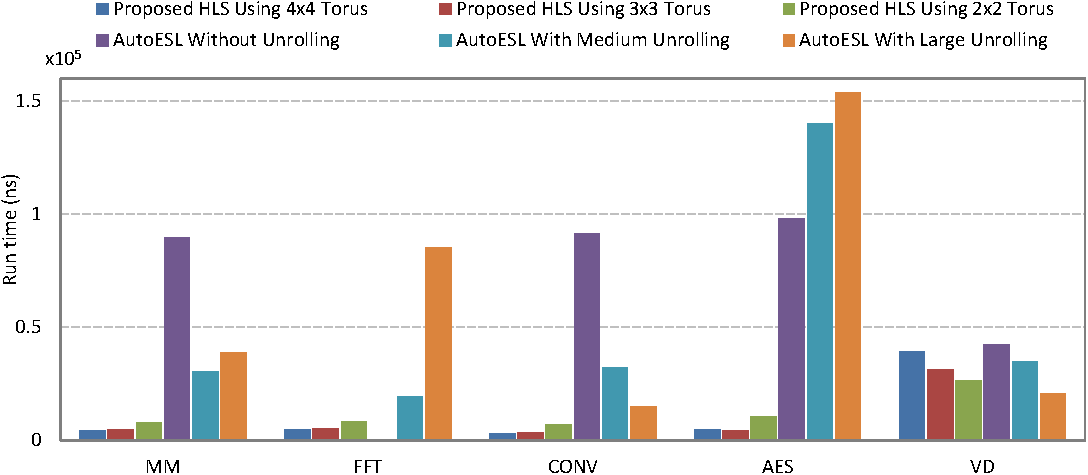
\includegraphics[width=8cm]{real_perf}
\vspace{-1em}
\caption{Performance comparison of the benchmark using both \autoesl and the proposed HLS methodology}
\label{fig:real_perf}
\vspace{-1em}
\end{figure}

%\section{Limitations and Future Work}\label{sec:discussion}
While the current implementation of our proposed HLS methodology has demonstrated promising initial results, there are a number of limitations that must be acknowledged and possibly addressed in future work.

First and foremost, the proposed methodology is designed to synthesize parallel computing kernels to execute on FPGAs only. As such, it is not a generic methodology to perform HLS on random logic.  Furthermore, the proposed method is intended to serve as part of a larger HW/SW synthesis framework that targets hybrid CPU-FPGA systems. Therefore, many high-level design decisions such as the identification of compute kernel to offload to FPGAs are not handled in this work.

To maximize the amount of parallelism, loops are fully unrolled in the current implementation and thus the loop iterations in the kernels must be known at compile time. In the future, the degree of unrolling should be automatically determined based on the amount of available on chip resources. Since the scheduler depends on lock step execution, all the input data are assumed to be available whenever they are required and all the output data can always be accommodated by the store FIFO. As a result, the application with a large data set may require an extremely large input/output FIFO. In future, we may allow the SCGRA to be stalled to tolerate load/store latency variation and smaller load/store FIFO will be sufficient. 

Finally, on-chip ROM resources for instruction storage is our current resource limitation. We intend to alleviate this bottleneck in the future through the use of better instruction encoding schemes and instruction sequence reuse. Partial loop unrolling instead of fully loop unrolling as mentioned above will also help relieve this problem.

\section{Conclusions}\label{sec:conclusions}
In this paper, we have proposed a SCGRA based high-level synthesis (HLS) methodology for compiling computing kernels on FPGAs.  

By using an SCGRA as an intermediate compile step, the lengthy low-level implementation tool flow is reduced to a relatively rapid operation scheduling problem. The number of FPGA application debug cycles achievable per day is thus significantly increased, which contributes directly into higher application designers' productivity.

Despite the use of an additional layer of SCGRA on the target FPGA, the overall application performance is not necessarily compromised. Implementation with close to maximum clock frequency resulting from the highly regular structure of the SCGRA, in combination with an in-house scheduler that can effectively schedule operation to overlap with pipeline latencies are both contributing factors to such overall high performance. 

Compared to a conventional HLS methodology, experiments have shown that design compilation time is reduced by 10-100x while performance of the resulting application run time is improved by 0.8-21x.  The implementations resulting from the proposed HLS methodology consume more BRAMs but fewer SLICEs, LUTs, FFs and DSPs when compared to the conventional HLS implementations with relatively heavy loop unrolling.



\section{Introduction}
Improving general-purpose processing system is getting extremely 
difficult. More and more computer architects believe that the major 
improvements in cost-energy-performance will come from domain-specific 
hardware accelerators. Recent years have already seen a number of successful 
demonstrations utilizing domain specific hardware accelerators for critical 
domains of applications such as deep neural network \cite{Jouppi2017tpu, Li2017survey} 
database operations \cite{Wu2014q100} and graph processing \cite{Jun2016graphicionado, Ozdal2016energy}. 
In order to explore the hardware accelerator design, a hardware accelerator simulator 
is usually required. Indeed there are already many exisitng tools \cite{systemc, chisel} and 
models \cite{dramsim2, ramulator} that can be used to help with the hardware accelerator 
design, it is non-trivial to develop a hardware accelerator on top of these work. For instance, there 
is a lack of general public cycle-accurate memory models available in \cite{systemc, chisel} while 
\cite{dramsim2, ramulator} expose only primitive memory access interface and need to be further 
wrapped for an accelerator simulator. And a general accelerator simulator 
framework is highly desired for the hardware accelerator simulator development.

Despite the difference of the accelerator simulators, we argue that a general 
accelerator simulator design framework should have three common yet important 
features. First of all, it should provide memory models of various memory 
architectures. Basically memory is usually critical to the hardware accelerator 
and greatly affects the accelerator design. At the same time, memory techniques evolve rapidly 
over the years and novel memory architectures with distinct features emerge. In order to explore 
hardware accelerator design, various memory architectures needs to be evaluated. 
Secondly, it should provide abstract user-frinedly memory interfaces. Hardware accelerators 
usually have complex memory access patterns such as stream access, burst access as well as random access. 
Thus higher abstract memory access interface instead of primitive memory access interface should be provided. 
Thirdly, it should provide trade-off between simulation speed and precision. Hardware accelerators 
may have distinct simulation speed and precision requirements while exploring the hardware accelerator. 
For instance, some of the applications such as graph accelerators may process on a big data set. 
Low-level accurate memory model may result in extremely long simulation. Thus a simplified memory model 
should be used to obtain the general performance of the accelerators. For applications that are sensitive 
to the memory access latency, more accurate memory models are preferred.

There is still a lack of general accelerator simulator framework that fullfills 
all the three features mentioned above. To that end, we proposed a flexible hardware accelerator 
simulation framework to be reused for general hardware accelerator simulator development. Basically, it 
integrates ramulator supporting various memory architectures as the underlying memory model and thus allows 
hardware accelerator exploration over a broad range of memory architectures. In addition, abstract memory 
interfaces as well as memory content management are provided to faciliate the accelerator accessing 
the memory model. Finally, it also provides a mix of cycle-accurate memory model and simiplified 
analytical memory model obtained though sampling to compromise on simulation speed and accuracy.

The rest of the paper is organized as follows. Section 2 is the realted work, Section 3 presents 
the proposed accelerator simulation framework. Section 4 provides the experimental results 
and Section 5 concludes this paper.






\section{Background} \label{sec:background}
In this section, we will briefly introduce the high level FPGA design tools,
the widely used BFS algorithm and the baseline pipelined BFS structure 
as the background.

\subsection{High level FPGA design tools}
Despite the relatively good performance, 
the HDL based design typically results in low design productivity, large reuse, 
portability and maintenance cost as well as ease of use challenge. 
To address this problem, the FPGA vendors have started 
to offer high level programming options such as C/C++ and OpenCL, which makes 
it possible for the designers without much low-level circuit design 
experiences \cite{nimbix, xilinx-sdaccel, intel-opencl} 
to program the FPGAs efficiently. In addition, the accelerator 
described with high level languages preserves many software-like features 
such as portability, ease of maintenance and use. Considering the  
continuously growing FPGA resources and stringent time-to-market requirements, 
the high level FPGA design tools \cite{Nane2016hls-survey} get increasing popularity.

\subsection{BFS Algorithm}
BFS is a widely used graph traversal algorithm and it is the basic 
building component of many other graph processing algorithms. 
It traverses the graph by processing all vertices with the same distance from the 
source vertex iteratively. The set of vertices which have the same distance from the 
source is defined as frontier. The frontier that is under analysis in the BFS iteration 
is named as current frontier while the frontier that is inspected from current frontier 
is called next frontier. By inspecting only the frontier, BFS can be implemented efficiently 
and thus the frontier concept is utilized in many BFS implementations.

A widely used frontier based BFS algorithm implementation is named as 
level synchronous BFS \cite{attia2014cygraph, betkaoui2012reconfigurable, 
zhang2017boosting}. The basic idea is to traverse the frontier vertices 
and inspect the neighbors of the current frontier vertices to obtain the 
frontiers in next BFS iteration. Then the algorithm can start a new 
iteration with a simple switch of current frontier queue and next frontier queue. 
The algorithm ends when the frontier queue is empty.

\subsection{Baseline pipelined BFS}
The basic pipelined BFS structure with classical top-down traverse 
is presented in Figure \ref{fig:base-bfs}. It can be roughly 
divided into four pipeline stages. In the first stage, it reads 
frontier from memory. Then it passes the frontier to the second stage
via the OpenCL channel for further inspection. In the second stage, 
frontier neighbors will be inspected from the graph data. While the 
graph is stored as compressed sparse row (CSR) format which has a row 
pointer array (RPA) containing the edge index starting position of each 
vertex and a column index array (CIA) which is essentially the incoming/outgoing 
neighboring vertex indices, the second stage must go through the RPA read and 
CIA read sequentially. When the frontier neighbors are 
drained from memory, the second stage then forwards them to the third stage.
In the third stage, each neighboring vertex will be checked if it is 
already visited in previous BFS iterations. If the vertex is not visited, 
it will be considered as frontier in next BFS iteration. The corresponding 
vertex status will be set and the vertex index will be sent to the last stage.
In the last stage, the vertex indices of the next BFS frontier will be 
written to main memory and level of the frontier vertices will be updated.

\begin{figure}
\center{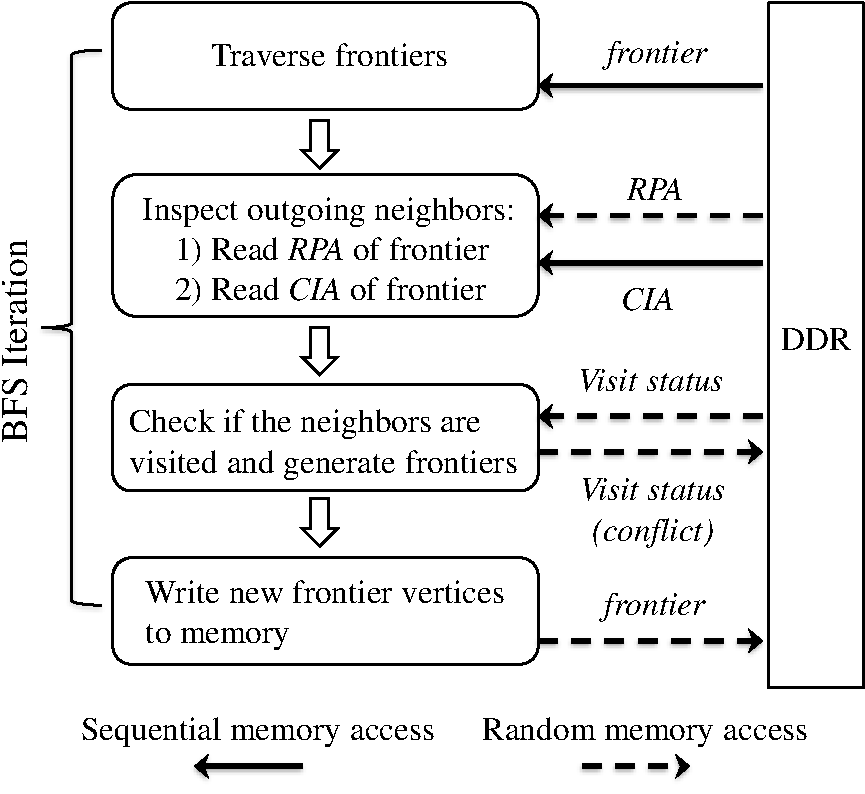
\includegraphics[width=0.7\linewidth]{base-bfs}}
    \caption{Baseline pipelined BFS}
\label{fig:base-bfs}
\vspace{-1em}
\end{figure}



\section{Resilient training framework} \label{sec:framework}
Resilient neural networks allow significant performance or 
energy efficiency improvement with little prediction accuracy penalty 
by relaxing the neural network accelerator design constraints. 
This motivates us to obtain more resilient neural networks 
for advantageous accelerator design trade-offs. 
A resilient neural network training framework will be 
detailed in this section. 

\subsection{Overall training framework}
For the problem that the computing error patterns are 
difficult to be captured in training with GPPs, 
we have the accelerators with computing errors integrated into 
the training process. Forward processing influenced by 
the accelerator computing errors is used in training directly 
such that computing error patterns and application data are 
reflected in the neural network models. For the problem that 
some of the layers are affected more than the others, 
we take these layers as critical layers and opt to 
protect the layers from being affected by computing errors. 
With reasonable performance penalty, we can improve the 
overall neural network resilience. 

Following this idea, the overall training framework is depicted in Figure \ref{fig:retrain}. 
Instead of training on GPPs, it has the majority of forward computing performed on the 
accelerators with computing errors while the rest of the training remains on GPPs.
Note that the critical layers should be executed on reliable hardware 
while GPP is one of the options. There are many different approaches 
that can be used to relax the design constraints.
Although they may cause distinct computing errors, they can be fitted to the 
same training framework.

\begin{figure}
        \center{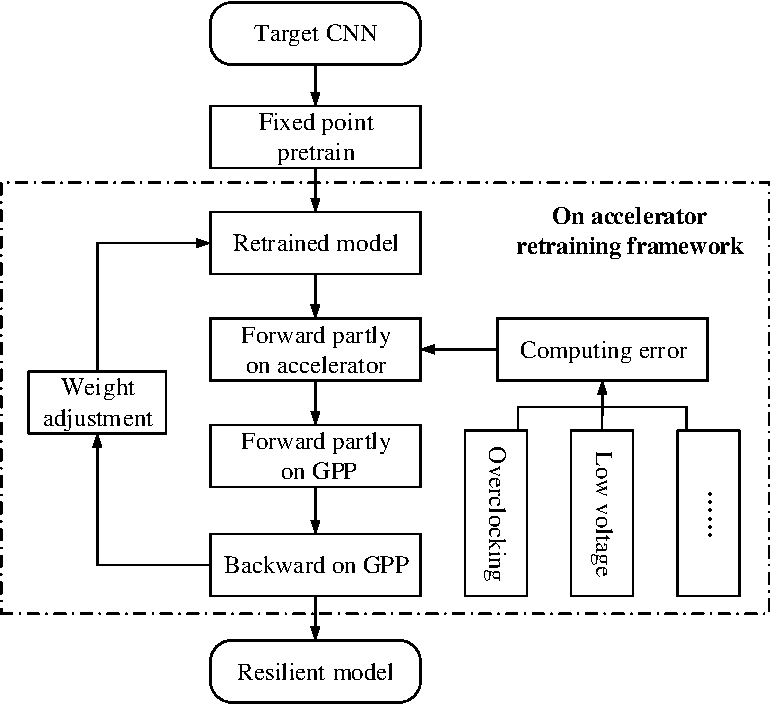
\includegraphics[width=0.85\linewidth]{on_accelerator_retrain_pocess}}
        \caption{Resilient neural network training framework}
        \label{fig:retrain}
        \vspace{-1em}
\end{figure}

\subsection{CNN accelerator abstraction and modification}
As illustrated in the above section, the forward propagation will 
mostly be executed on the CNN accelerator while 
the rest part runs on GPPs. Essentially, the framework targets at a 
heterogeneous computing architecture and frequent 
communication between the accelerator and the GPPs are expected. 
In order to fit various CNN accelerators within the same training framework,
we abstract the CNN accelerators with a high-level interface
which makes the accelerators near transparent to the training framework.
To facilitate the data communication between the forward propagation
and the rest of the training framework, we define a high-level
interface which consists of 7 functions as listed inTable \ref{tab:api}.
%Function 1 is used to launch the CNN accelerator from host. 
%Function 2 and 3 are used to transfer data between the host memory and the device memory during 
%the training. As the forward propagation on the CNN accelerators is usually fixed point 
%and the back propagation on GPPs is floating point, data type converting between fixed point 
%and floating point is required. Function 4 and 5 can be used for this purpose. 
%Function 1 to 5 are required for all the accelerators. 
%Function 6 and 7 are only used for accelerators that compute on reorganized data\cite{pipecnn_2,deepburing_12}. 
With the interface functions, general CNN accelerators can be conveniently
referenced and used in the proposed on-accelerator training framework.
\begin{table*}
	\
        \centering
        \vspace{-0.3em}
        \caption{High-level interface to integrate general CNN accelerators with Caffe}
        \label{tab:api}
        \vspace{-0.3em}
        \begin{tabular}{c|l|l}
                \toprule
                ID & Function Name & Description  \\
                \midrule
                1 & launchAccelerator() & It configures the CNN accelerator and launches it from host CPU. \\
		\midrule
                2 & dataToFPGA(weight, input, wgtDevAddr, inDevAddr) & It transfers both the input data and weight to the FPGA device memory. \\
		\midrule
		3 & dataFromFPGA(outputDevAddr, output) & \shortstack[l]{It transfers intermediate data from FPGA device memory to host memory.} \\
		\midrule
		4 & convertIntToFloat(int iData, float fData) & It converts the fixed-point point to float for back propagation processing. \\
		\midrule
		5 & convertFloatToInt(float fData,  int iData) & \shortstack[l]{It converts the floating-point input and weight to fixed point for forward processing.} \\
		\midrule
		6 & dataLayoutReorder(data, reorderedData) & \shortstack[l]{It reorders the data layout for more efficient accelerator execution.} \\
		\midrule
		7 & dataLayoutRecover(reorderedData, data) & It reorders the output data back to the default format for Caffe back propagation. \\
                \bottomrule
        \end{tabular}
        \vspace{-1em}
\end{table*}

In this work, we have the CNN accelerator implemented on Xilinx FPGAs as a case study. 
With Xilinx SDAccel, we can wrap the accelerators with OpenCL API while the accelerators 
can either be developed with OpenCL, HLS or RTL. On top of the OpenCL API, the proposed 
high-level interface can be implemented. Meanwhile, we use Caffe, a C++ based 
deep learning framework, to construct the on-accelerator training framework. With 
both parts developed with C family languages, they can be integrated conveniently. 

%In this work, we have the CNN accelerator implemented on FPGAs.
%Figure 4 depicts the implementation of the training framework on a hybrid 
%CPU-FPGA architecture. In this work, we use Xilinx KCU1500 as the FPGA board 
%and put it on a standard desktop computer. CPU is the controller and it reconfigures 
%the accelerator for a specific CNN structure. In each training iteration, CPU launches 
%the CNN accelerator to perform the forward propagation from bottom layer to top layer. 
%CPU does the backward propagation from top layer to bottom layer. Weights and the image 
%data are initially stored in host memory. It will be transferred to FPGA offchip memory 
%for forward propagation through PCI-E. Similarly, the output data will be transferred 
%from FPGA off-chip memory back to host memory after forward propagation. Because of the 
%OpenCL based API wrapper in SDAccel, the CNN accelerator’s interface can be easily 
%exposed to Caffe for referring to the forward propagation result. 

\begin{figure}
        \center{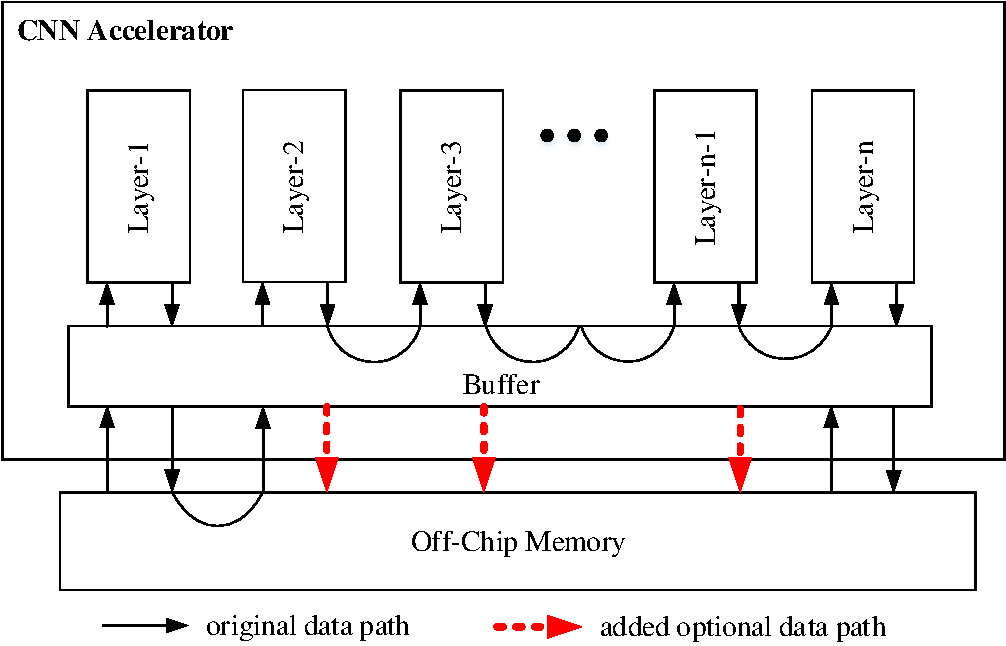
\includegraphics[width=0.85\linewidth]{change_of_accelerator}}
        \caption{Modification of the CNN accelerator data path. It essentially
ensures the feature map of each neural network layer to have an optional data path
to external memory for back propagation in training.}
        \label{fig:change_of_accelerator}
        \vspace{-1em}
\end{figure}

On top of the high-level interface, the CNN accelerator also needs 
minor modification to enable the on-accelerator training. 
The training requires the feature map of each neural 
network layer for backward propagation. However, many of the accelerators 
are intensively optimized for inference only and some of the layers' output 
are fully buffered in on-chip memory to reduce the external memory access. 
Thereby, the accelerator should provide an optional data path such that 
intermediate output data can be written to external memory at request.
As shown in Figure \ref{fig:change_of_accelerator}, the output of each layer 
will be transferred to memory using the added data path 
when the accelerator is used for training. The write back data path 
can be switched off during inference. 

\subsection{Critical neural network layer protection}
In order to improve the overall neural network resilience, we opt to 
protect the critical network layers to alleviate the resilience 
bottleneck. The protection is essentially 
to have the critical layers executed on reliable computing infrastructures 
and the exact protection method depends on the target hardware platform.
We may either schedule the critical layers to the GPPs or switch the accelerator 
to reliable mode during the execution of the critical layers.
With this approach, the overall network can tolerate 
more computing errors. 

To decide the critical layers of the neural networks, we formulate the 
critical layer selection scheme. Suppose the neural network layers include 
$N$ layers and each layer is represented as $L_i$ where $i \in {0, 1, 2, ..., N-1}$.
Then we evaluate the prediction accuracy loss of the neural network 
that have one layer protected on accelerators with computing errors.
When the $i$th layer is protected, the loss is $loss_i$.
Then the most critical layer is the layer that leads to the most 
accuracy loss i.e. $c \in \{k|loss_k = max(loss_i), i \in \{0, 1, ..., N-1\}\}$.

The above formulated approach requires large amount of evaluation of 
different layers of the neural network. Instead, we use the actual 
computing errors as the critical layer selection metric. We set an 
error threshold $T$ and assume 8bit integers are used. 
When the error equals to 0, the computing results are correct. 
When the error is larger than $T$, the results are assumed to be large errors.
When the computing results are wrong but smaller than $T$, the results are considered 
as moderate errors. The layers that include the largest portion of large errors 
are taken as the critical layers.

In addition, scheduling the neural network layers executed 
on the accelerator to GPPs has performance penalty due to the 
computing efficiency gap. As the accelerators are usually 
orders of magnitudes faster than the GPPs for neural network 
processing especially large convolution layers, we can focus on 
the last few small layers to ensure negligible performance 
loss. This constrain greatly reduces the search space
of the critical layers. 



\section{Experiments and results} \label{sec:result}
The experiments mainly include two parts. In the first part, we 
analyze the implementations of the SCGRA overlay based FPGA accelerators with 
different configurations to demonstrate the regularity of the 
SCGRA overlay based FPGA accelerators. In the second part, we benchmark the 
efficiency and quality of the proposed customization framework.

\subsection{Experiment Setup}
All the run time was obtained from a computer with Intel(R) Core(TM) 
i5-3230M CPU and 8GB RAM. Zedboard which has an ARM processor and 
an FPGA was used as the hybrid computation system. Vivado 2013.3 was 
used for the HLS based design and PlanAhead 14.7 was used for the SCGRA overlay based 
design. 

The overlay implementations on Zedboard typically run at 200MHz and we 
assume the implementation frequency can be scalable to all the 
different overlay configurations. The power consumption used in this work was 
obtained from XPower which is part of the Xilinx design suite.

\subsection{SCGRA Overlay Implementation Analysis}
In order to analyze the overhead and power of the SCGRA overlay 
based FPGA accelerators, we had three groups of accelerators 
(SCGRA1, SCGRA2, SCGRA3) implemented on Zedboard. The configurations 
are detailed in \tabref{tab:config}. Despite of the diverse 
configurations, all the implementations could meet 200MHz 
timing constrain. With this timing constrain, 
hardware overhead and power consumption are analyzed in the 
following sub sections.
\begin{table}[tb]
    \small
    \centering
    \caption{SCGRA Based FPGA Accelerator Configuration \label{tab:config}}{
        \begin{tabular}{c|c|c|c|c|c}
            \hline
            Group & Size & \tabincell{c}{Inst. \\ Rom} & 
            \tabincell{c}{Data \\ Mem} & \tabincell{c}{IBuf \\ /OBuf} & 
            \tabincell{c}{Addr \\Buf} \\ \hline

            SCGRA1 & \tabincell{l}{2x2, 3x2, \\ 3x3, 4x3, \\ 4x4, 5x4} & 
            1kx72 & 256x32 & 2kx32 & 4kx16\\ \hline

            SCGRA2 & \tabincell{l}{2x2, 3x2, \\ 3x3, 4x3, \\4x4} & 
            2kx72 & 256x32 & 2kx32 & 4kx16\\ \hline

            SCGRA3 & \tabincell{l}{2x2, \\ 3x2, \\ 3x3 } &  
            4kx72 & 256x32 & 2kx32 & 4kx16\\ \hline
        \end{tabular}
    }
\end{table}

\subsubsection{Hardware Overhead}
\figref{fig:SCGRA-Overhead} shows the relation between 
the four types of hardware resource overhead and SCGRA 
overlay size. It can be found that FF, LUT and DSP overhead 
do not change much with the memory configurations and they 
present good linearity to the overlay size, thus they can be 
estimated with linear models. BRAM overhead depends 
on both the overlay size and the memory configurations, 
and single variable linear model will not work for the estimation.
Fortunately, it can be calculated precisely with the memory 
configurations. 

\begin{figure}[tb]
    \subfloat[\label{fig:FF-Overhead}]{%
      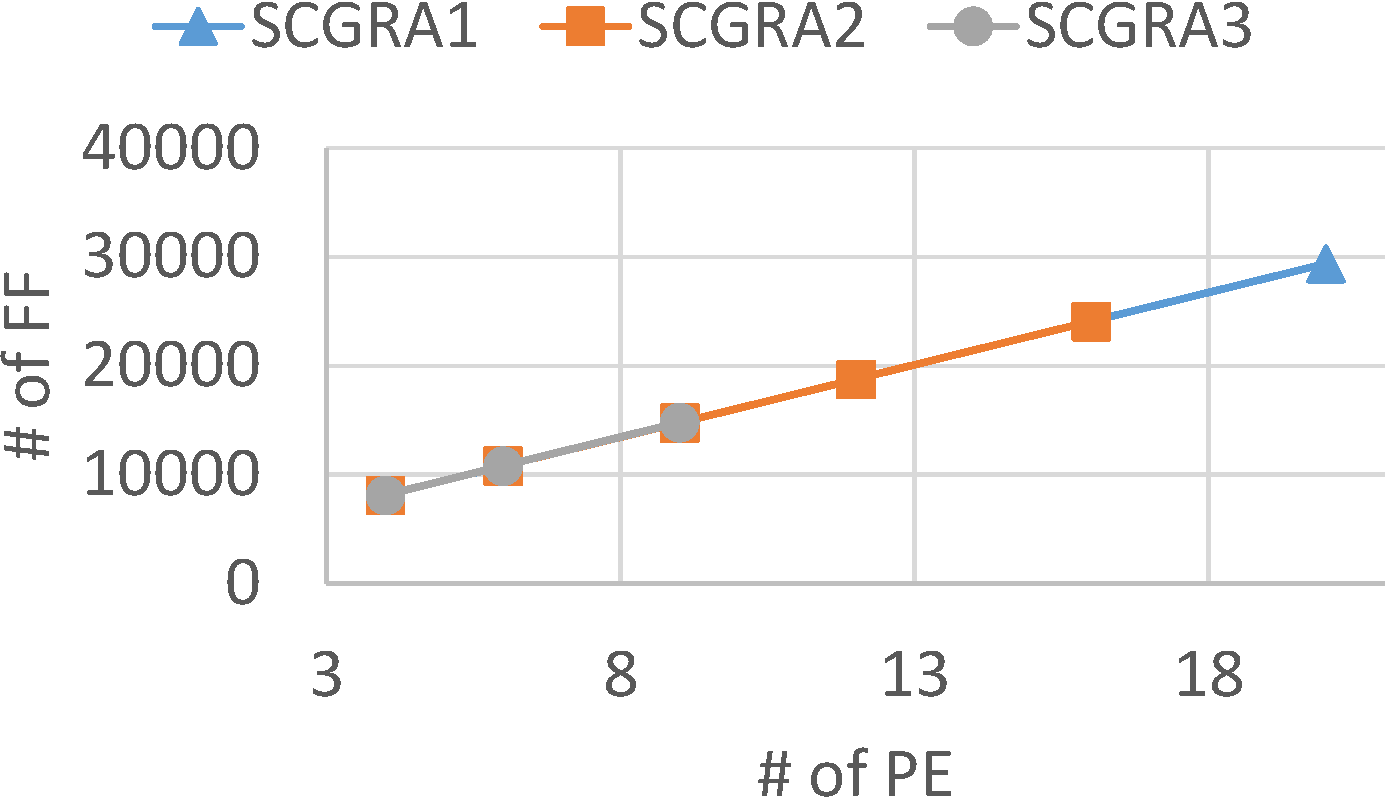
\includegraphics[width=0.22\textwidth]{FF-Overhead}
    }
    \subfloat[\label{fig:LUT-Overhead}]{%
      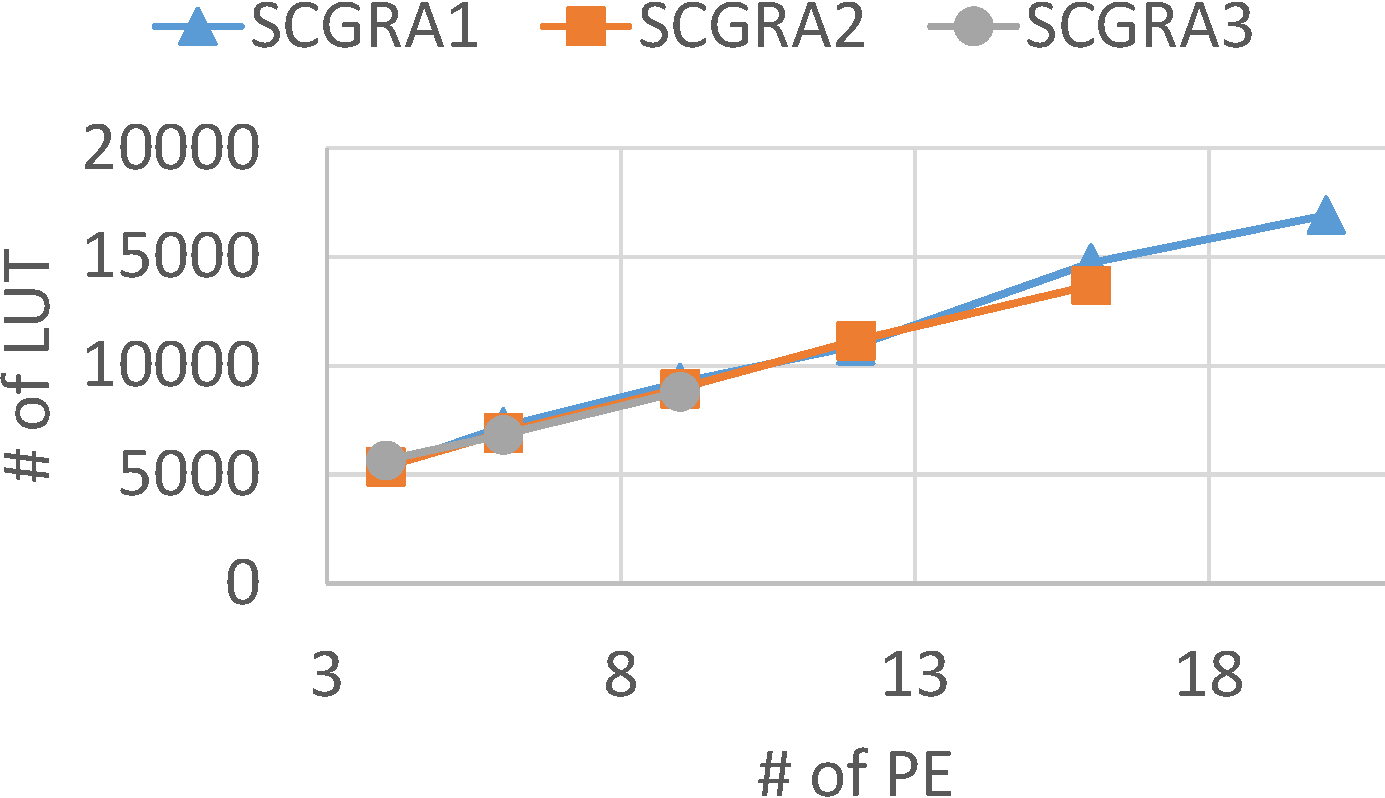
\includegraphics[width=0.22\textwidth]{LUT-Overhead}
    }
    \hfill
    \subfloat[\label{fig:DSP-Overhead}]{%
      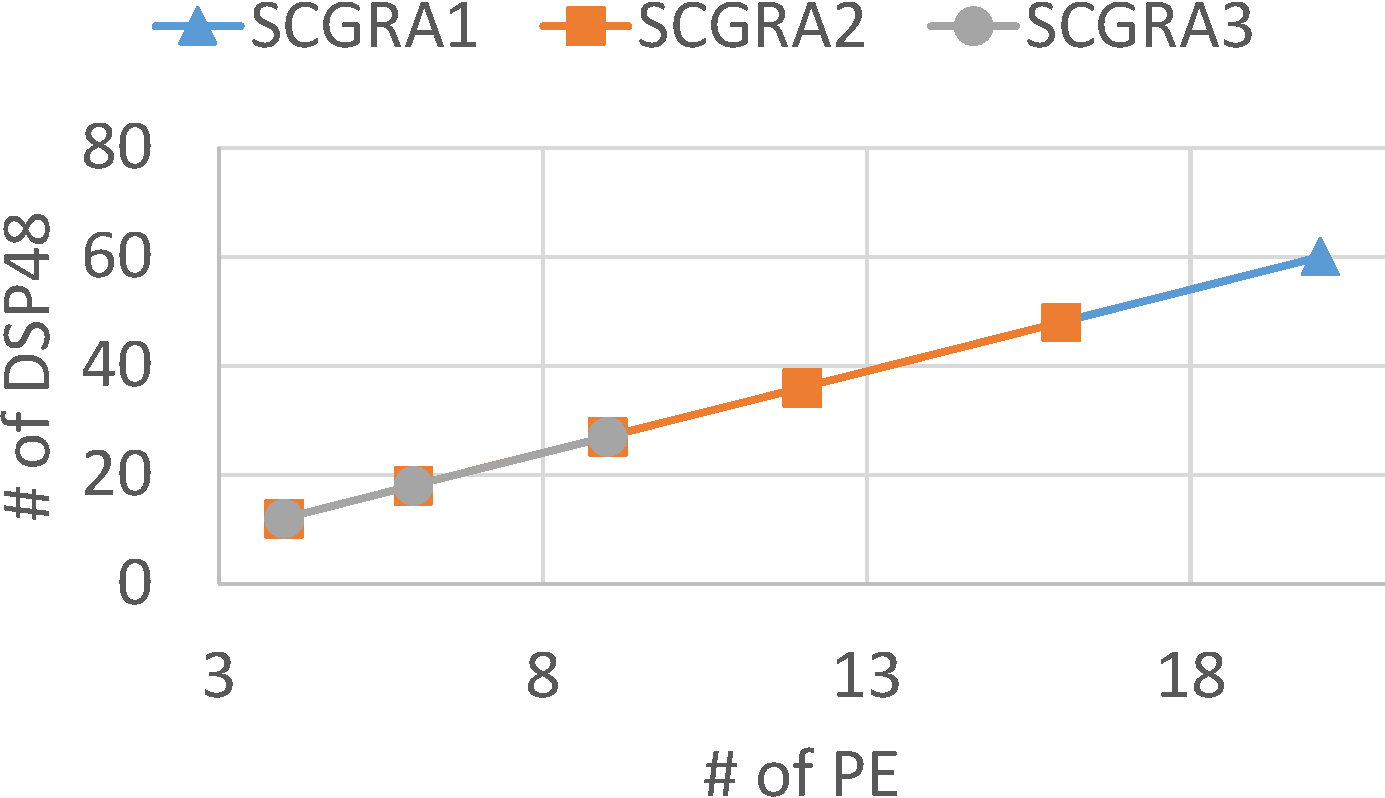
\includegraphics[width=0.22\textwidth]{DSP-Overhead}
    }
    \subfloat[\label{fig:BRAM-Overhead}]{%
      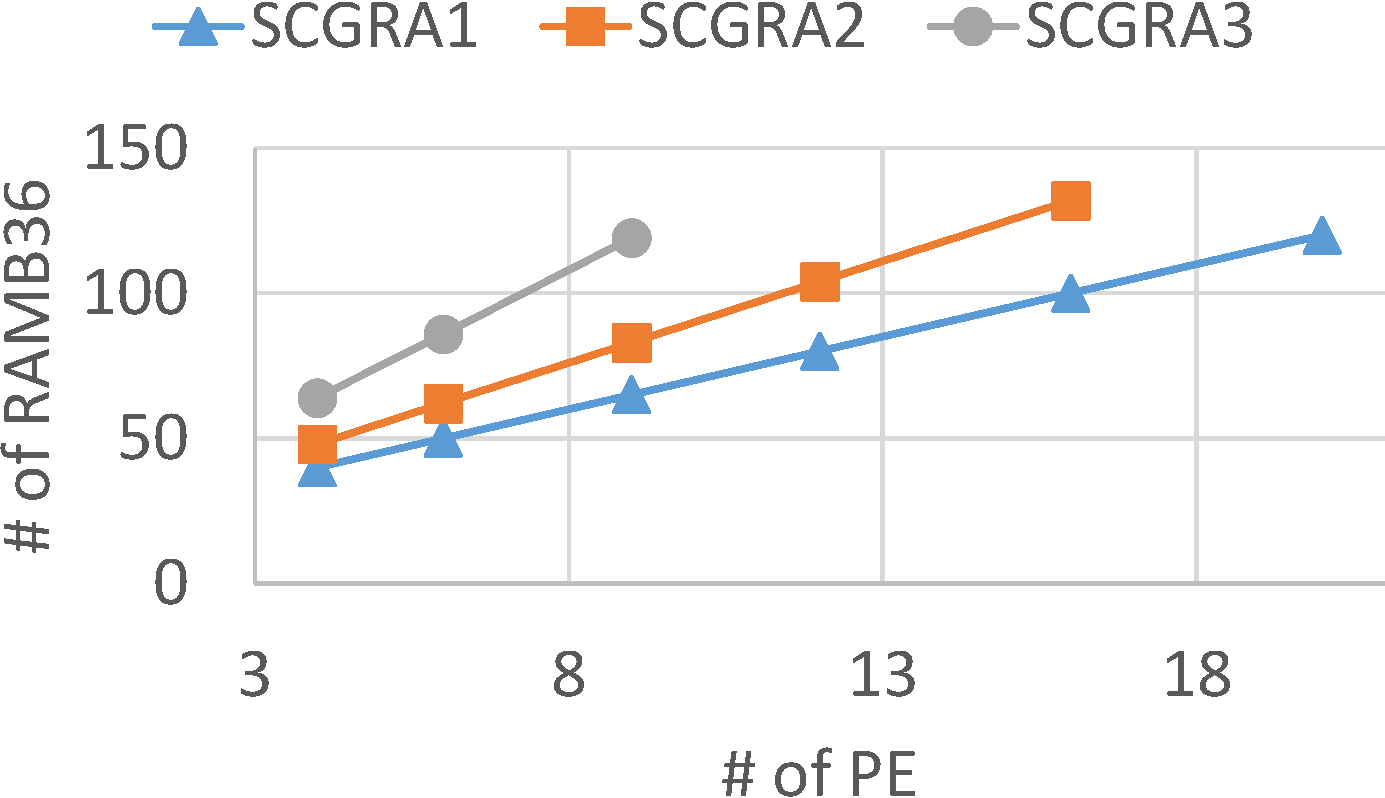
\includegraphics[width=0.22\textwidth]{BRAM-Overhead}
    }
    \caption{Relation between the accelerator overhead and overlay size, 
    (a) FF overhead, (b) LUT overhead, (c)DSP overhead, (d)BRAM overhead}
    \label{fig:SCGRA-Overhead}
\end{figure}


\subsubsection{Power Consumption}
According to the power decomposition in Xpower, the power consumption 
of an FPGA design includes signal power, clock power, BRAM power and so on. 
To simplify the power model of the SCGRA overlay based FPGA accelerator, 
we divide the power consumption into BRAM power and base system 
power which essentially includes the power consumption of the rest part of the system. 
As shown in \figref{fig:SCGRA-Power}, the base system power exhibits good linearity 
over the SCGRA overlay size while the BRAM power is near linear to 
the BRAM overhead. Therefore, both of them can be easily estimated with linear models. 

\begin{figure}[tb]
    \subfloat[\label{fig:Base-Power}]{%
      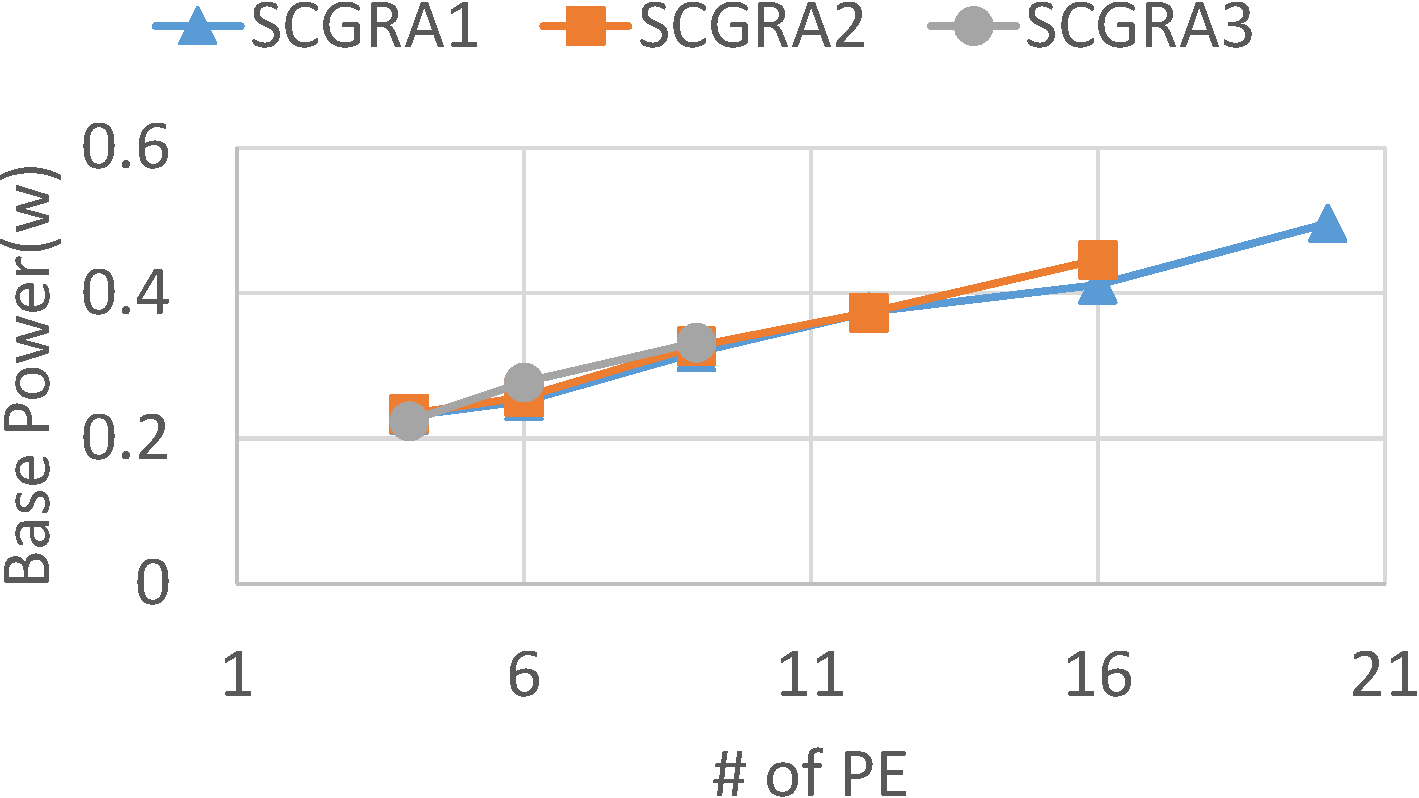
\includegraphics[width=0.22\textwidth]{Base-Power}
    }
    \subfloat[\label{fig:BRAM-Power}]{%
      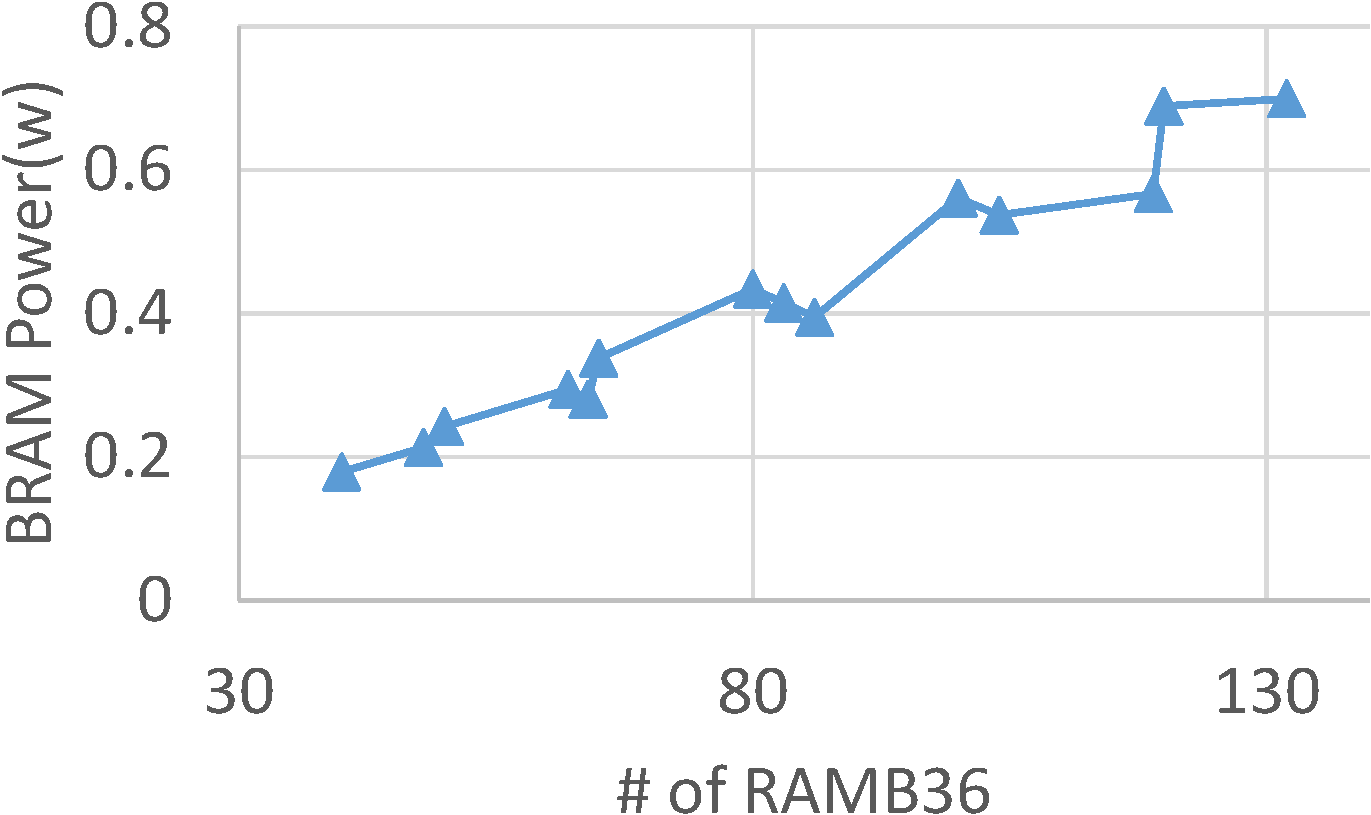
\includegraphics[width=0.22\textwidth]{BRAM-Power}
    }
    \caption{Power consumption of the SCGRA overlay based FPGA accelerator, 
    (a) Base system power including DSP power, clock power, etc., (b) BRAM power}
    \label{fig:SCGRA-Power}
\end{figure}

\subsection{Proposed Design Framework Evaluation}
In this work, we take four applications including Matrix Multiplication (MM), 
FIR, Kmean(KM) and Sobel Edge Detector (SE) as our benchmark. The 
configurations of the benchmark are detailed in \tabref{tab:benchmark-config}. 
In order to evaluate the efficiency and quality of the proposed design 
framework, we have the benchmark implemented using both the proposed 
two-step customization (TS) method and an exhaustive search (ES) 
method. Then we compared the Pareto-optimal curves acquired 
using both methods. In addition, we also have the benchmark 
implemented using Vivado HLS with moderate manual optimization 
and compare the implementations with our customized implementations. 

\begin{table}[tb]
    \small
    \centering
    \caption{Benchmark Configurations \label{tab:benchmark-config}}{
        \begin{tabular}{l|l|l}
            \hline
            Benchmark & Parameters & Loop Structure \\ \hline
            MM & Matrix Size(128) & $128 \times 128 \times 128$ \\ \hline
            FIR & \tabincell{l}{\# of Input (1024) \\ \# of Taps+1 (64)} & $1024 \times 64$ \\ \hline
            SE & \tabincell{l}{ \# of Vertical Pixels (128) \\ \# of Horizontal Pixels (8)} & $128 \times 8 \times 3 \times 3$ \\ \hline 
            KM & \tabincell{l}{\# of Nodes(1024) \\ \# of Centroids(4) \\ \# of Dimensions(2)} & $1024 \times 4 \times 2$ \\ \hline  
        \end{tabular}
    }
\end{table}

\subsubsection{Customization Methods Comparison}
\figref{fig:DSE-Time} shows the DSE time of both the TS DSE and ES DSE. 
The proposed TS DSE is around 100x faster than the ES DSE on 
average. In particular, it can be found that ES DSE can be 
extremely slow on MM which has three levels of loop with relatively large 
loop count and thus larger design space. Though TS DSE also needs 
longer time to complete the DSE of MM, it can skip most 
of the unfeasible configurations and the runtime is 
less sensitive to the size of the design space. 

\begin{figure}[tb]
    \centering
    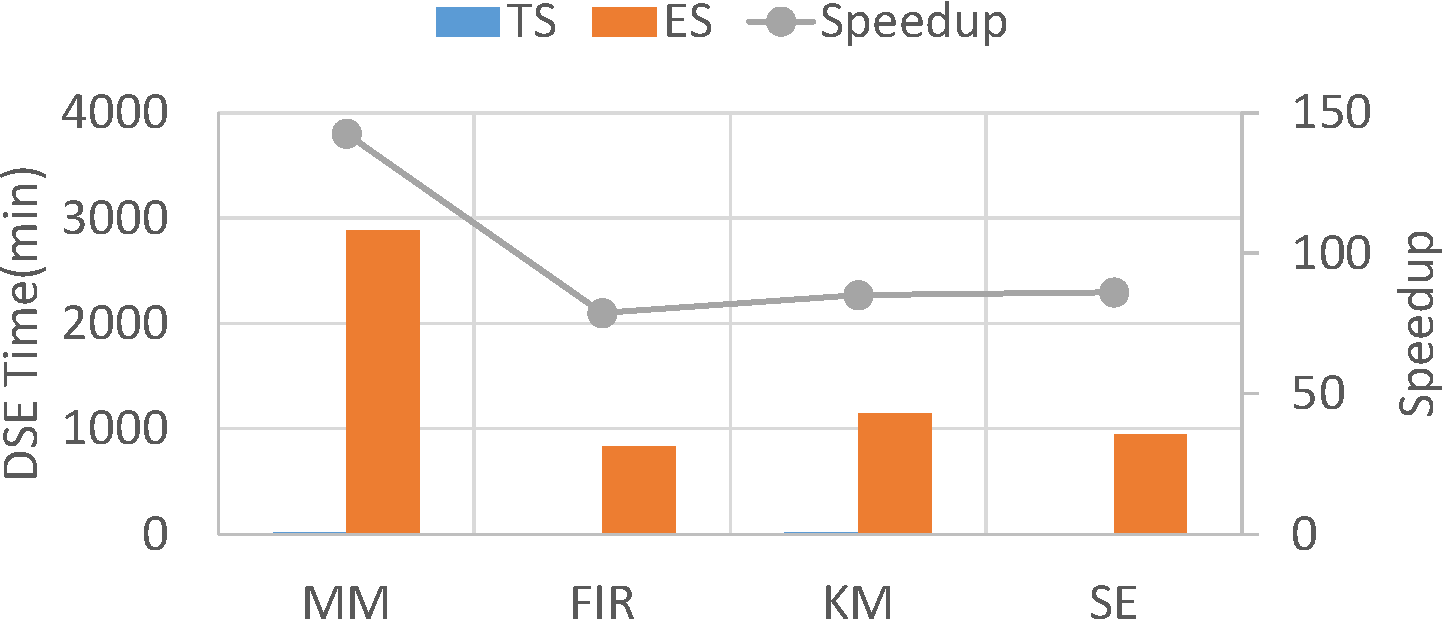
\includegraphics[width=0.35\textwidth]{DSE-Time}
    \caption{DSE time of the benchmark using both TS and ES}
    \label{fig:DSE-Time}
\end{figure}

%\begin{table}[tb]
%    \small
%    \centering
%    \caption{Time Cost for RA DSE and ES DSE\label{tab:dsetime}}{
%        \begin{tabular}{l|l|l|l|l}
%            \hline
%            Benchmark & MM & FIR & KM & SE \\ \hline
%            RA DSE (min) & 20.2 & 10.6 & 13.4 & 11.4\\ \hline
%            ES DSE (min) & 2880.6 & 835.2 & 1140.5 & 946.2\\ \hline
%            Speedup & 142.6 & 78.8 & 85.1 & 86.2 \\ \hline
%        \end{tabular}
%    }
%\end{table}

In order to demonstrate the quality of proposed framework, we presented the 
Pareto-optimal curves acquired from both DSE methods as shown in \figref{fig:DSE}. 
It is clear that the Pareto-optimal curves obtained via the two DSE methods are quite 
close. Since TS DSE may prune the design options that involve a larger 
overlay size and better performance according to the sub DSE metric, 
the Pareto-optimal curves may deviate slightly at the higher performance area. 
Fortunately, this can be improved by lowering user defined metric $\epsilon$ 
while affording longer DSE time. When we customize the design for minimum energy 
consumption, TS DSE can achieve the optimal design in all the benchmarks. 

\begin{figure}[tb]
	\subfloat[MM]{%
		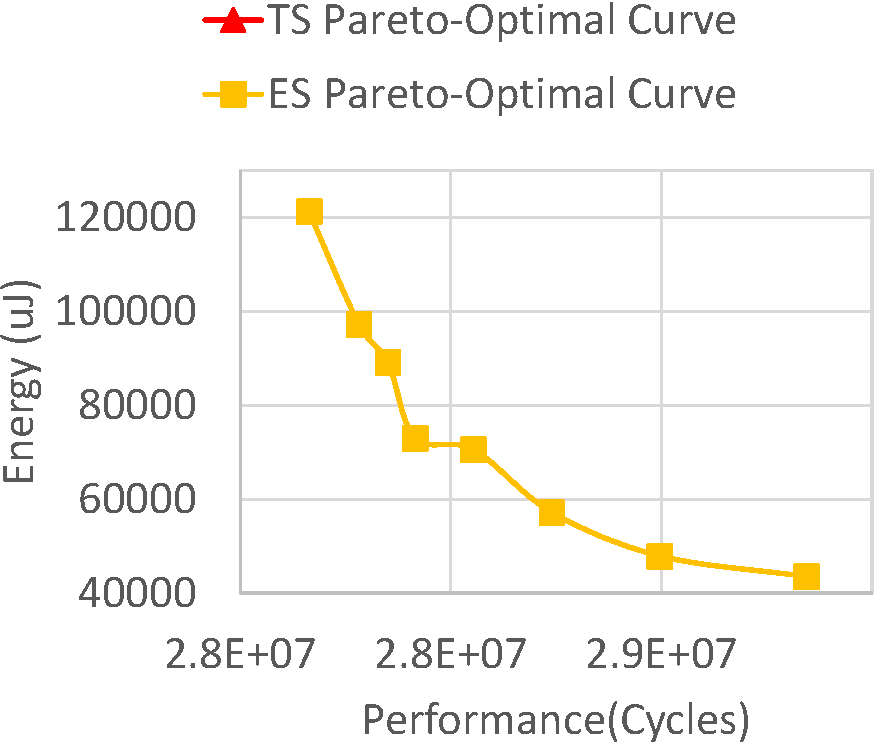
\includegraphics[width=0.22\textwidth]{mm-energy-performance}
	}
	\subfloat[FIR]{%
		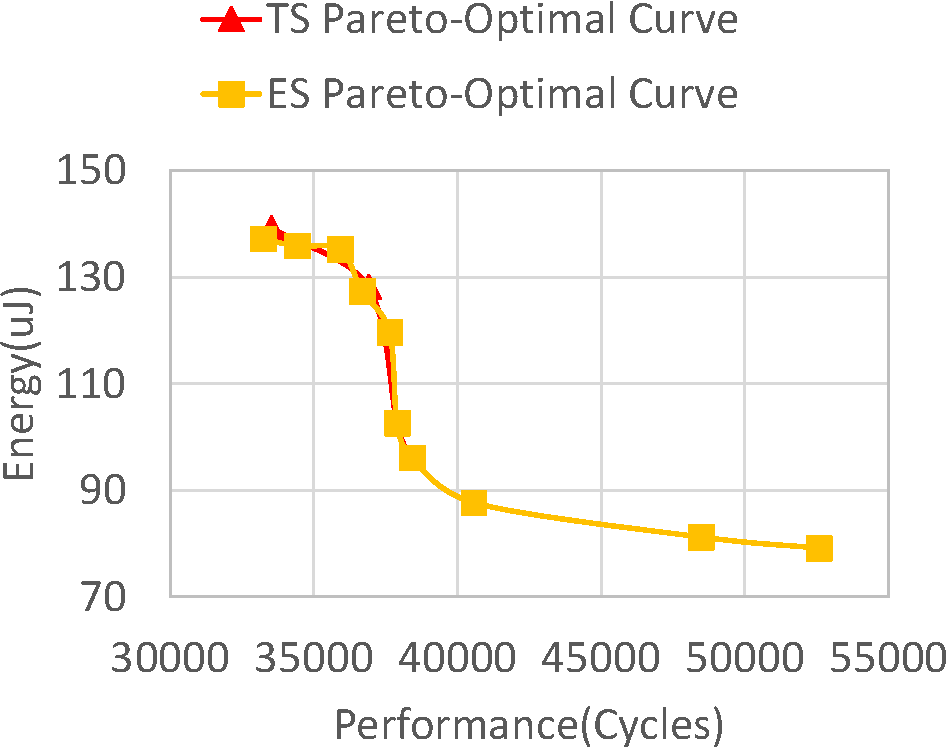
\includegraphics[width=0.22\textwidth]{fir-energy-performance}
	}
    \hfill
	\subfloat[SE]{%
		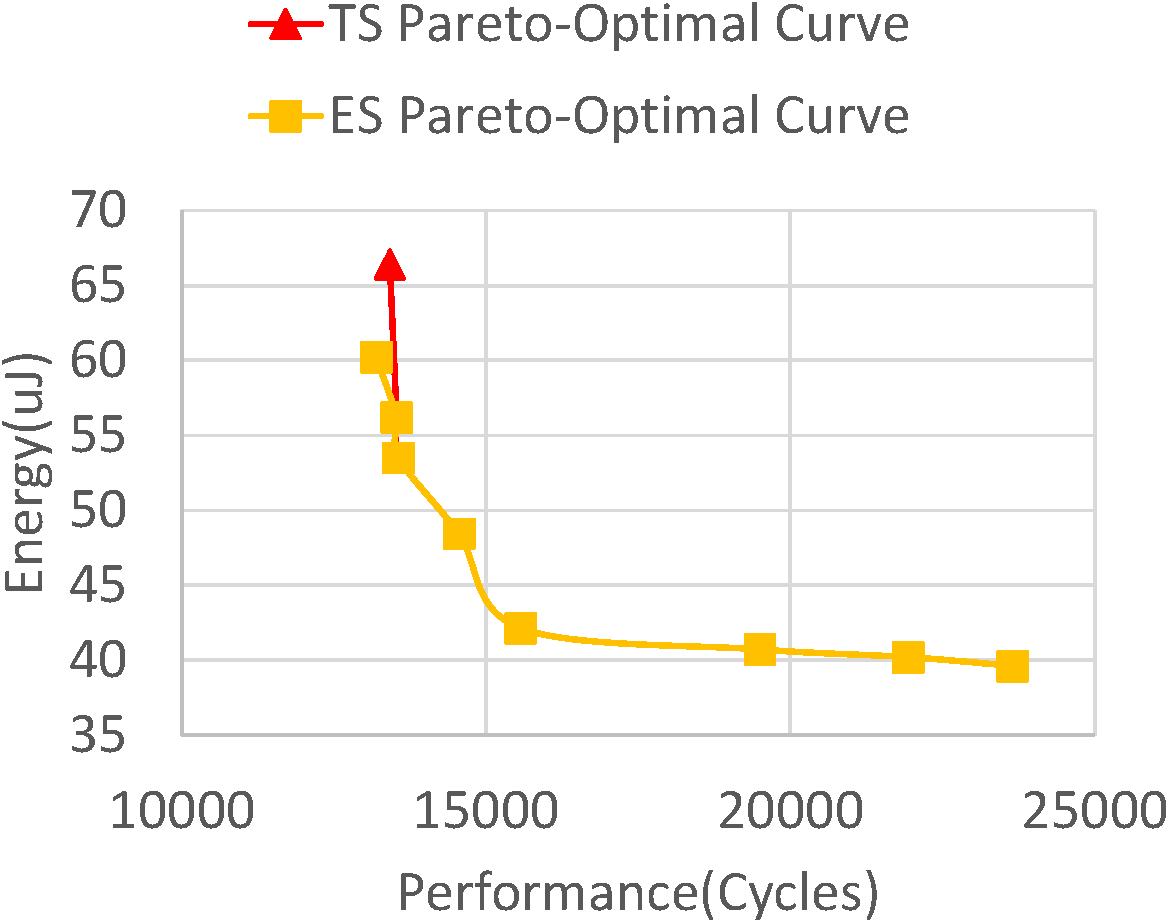
\includegraphics[width=0.22\textwidth]{se-energy-performance}
	}
	\subfloat[KM]{%
		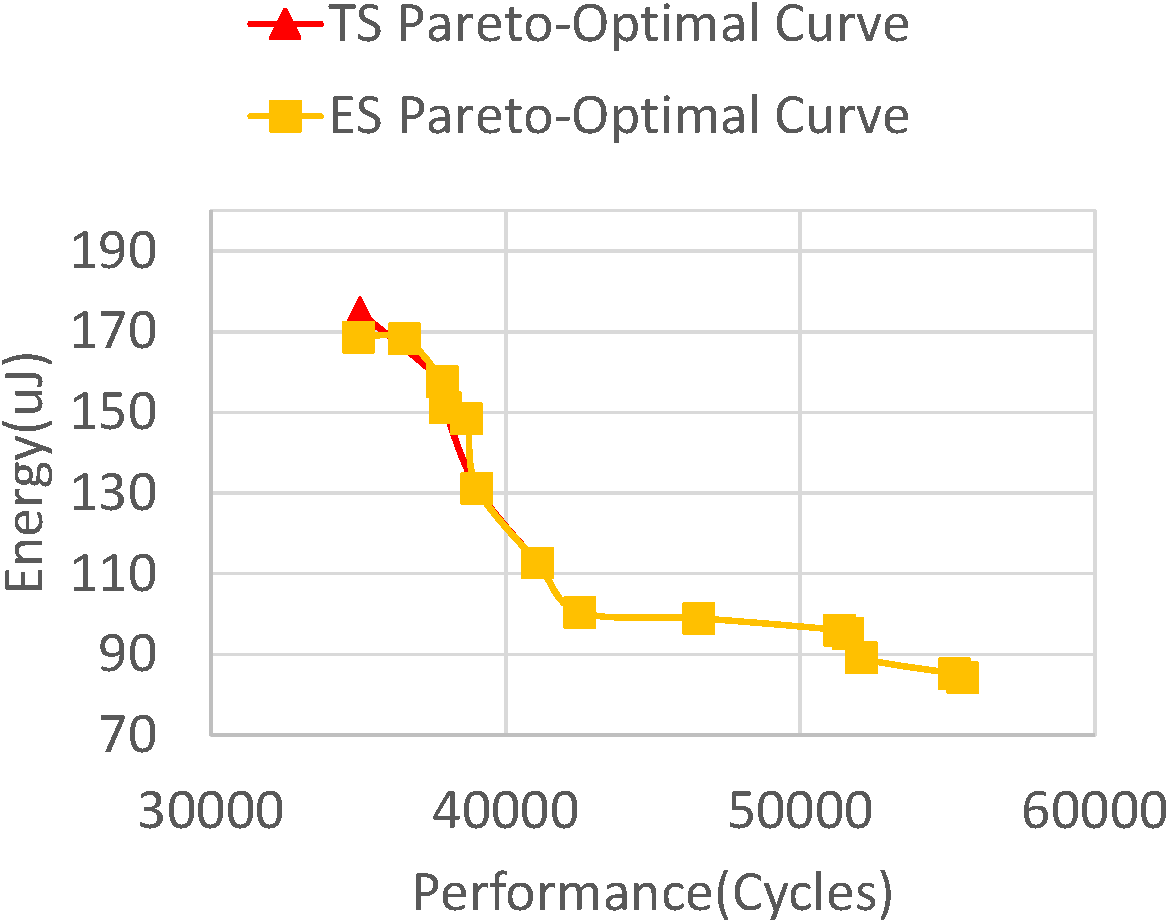
\includegraphics[width=0.22\textwidth]{km-energy-performance}
	}
    \caption{Performance-Energy Pareto-optimal curve}
	\label{fig:DSE}
\end{figure}

\subsubsection{Design Tools Comparison}
The proposed design framework will not be as useful if the performance of the 
generated system is not at least on par with similar systems created with 
conventional high-level synthesis tools. For that, we further implemented the 
benchmarks using Vivado HLS with moderate effort. The loops in the benchmark will 
be unrolled as much as possible and the input/output buffers are set as large 
as possible. Then the accelerators generated using both tools are compared. 
Since similar comparison has already been done in previous work \cite{scgra-orig}, 
we just brief the performance comparison for a quick reference.

\begin{figure}[tb]
	\subfloat[MM]{%
		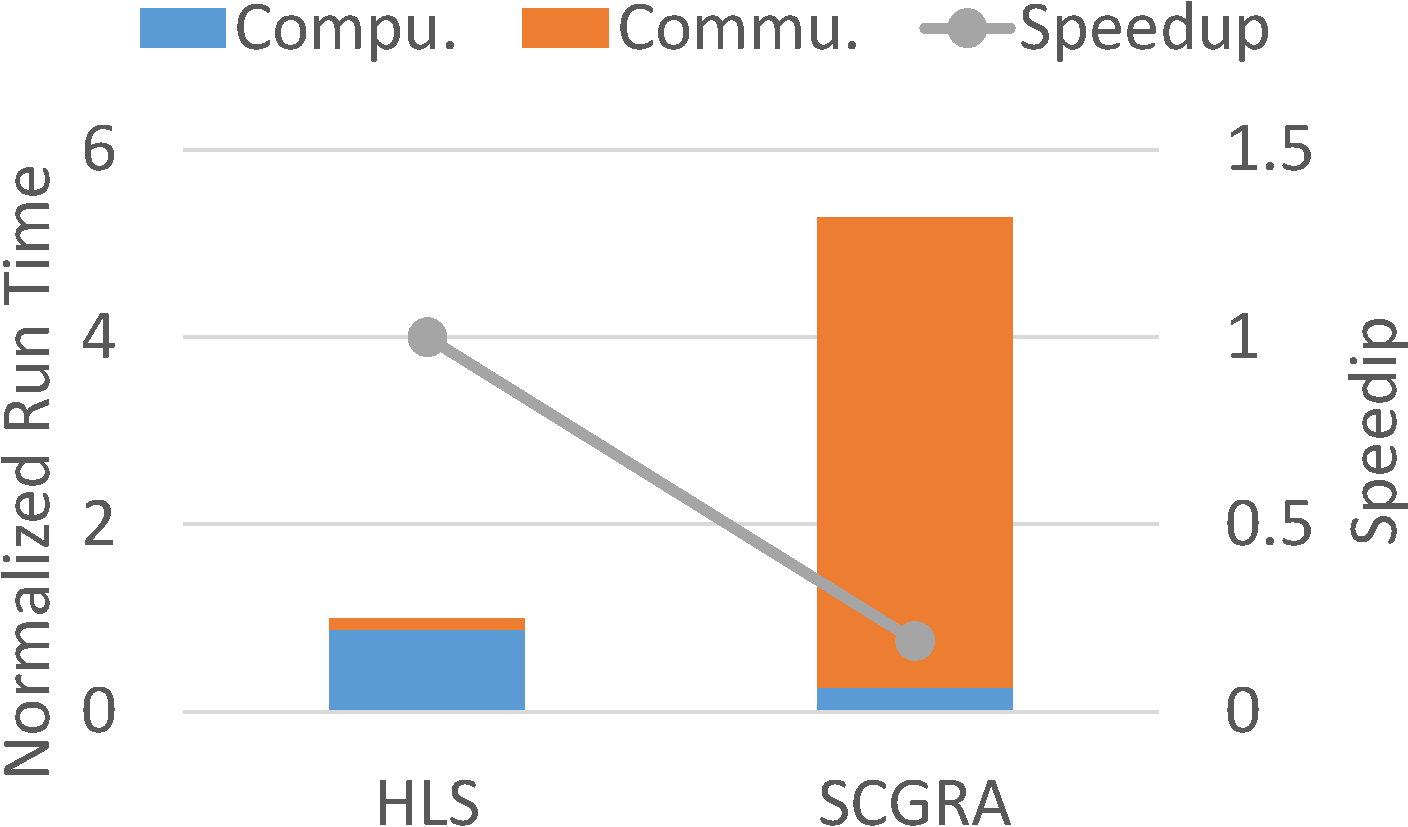
\includegraphics[width=0.22\textwidth]{mm-hls-cp}
	}
	\subfloat[FIR]{%
		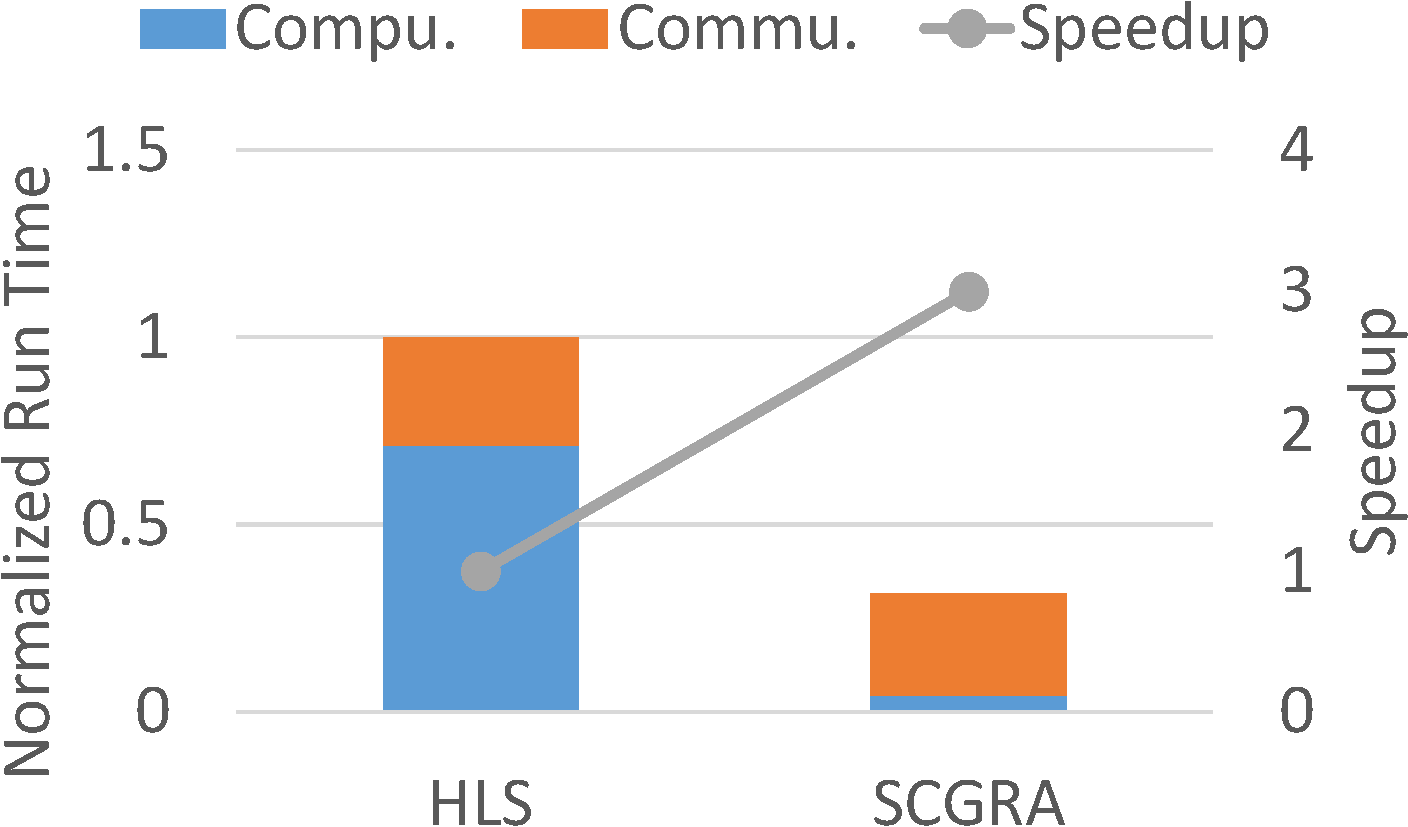
\includegraphics[width=0.22\textwidth]{fir-hls-cp}
	}
    \hfill
	\subfloat[SE]{%
		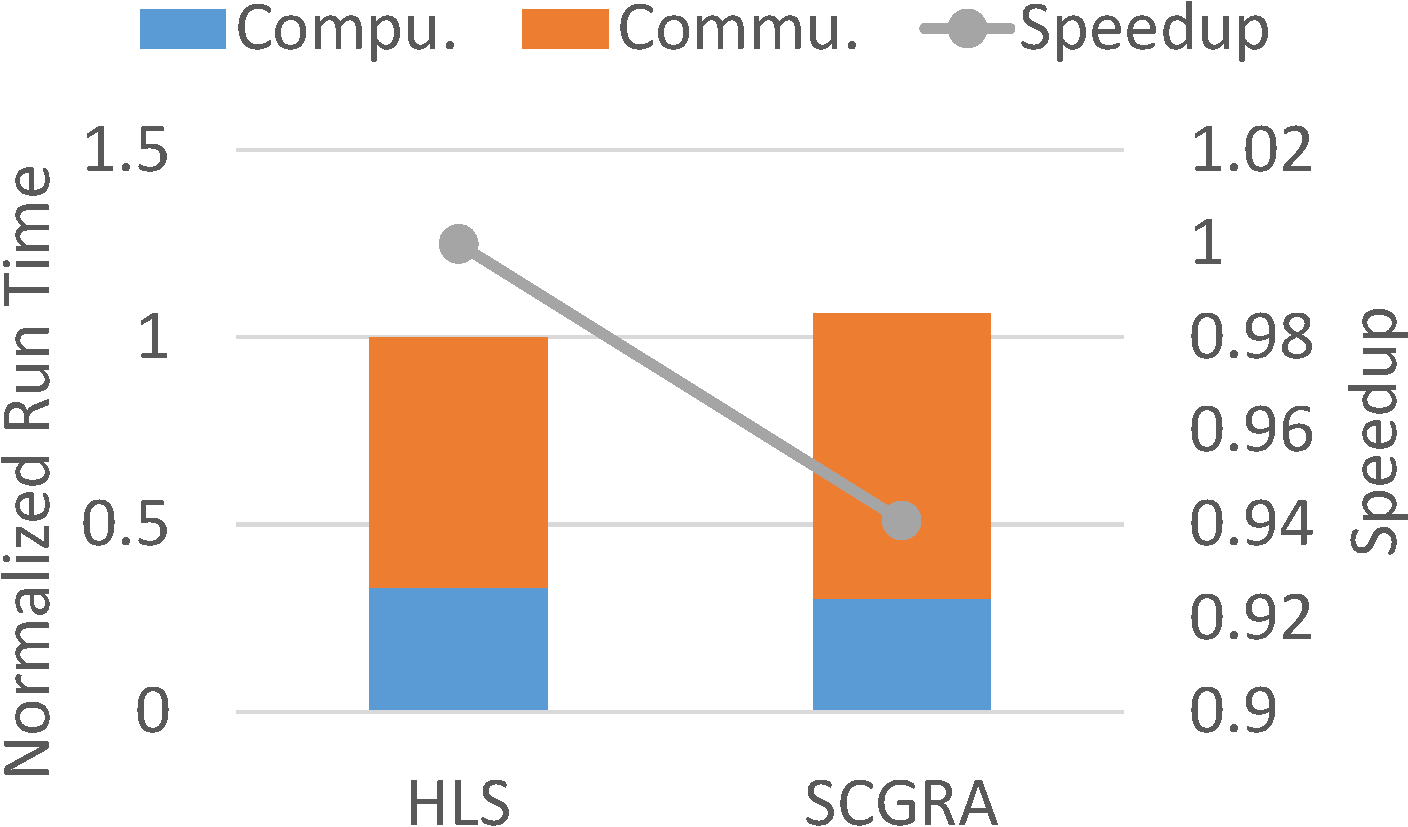
\includegraphics[width=0.22\textwidth]{se-hls-cp}
	}
	\subfloat[KM]{%
		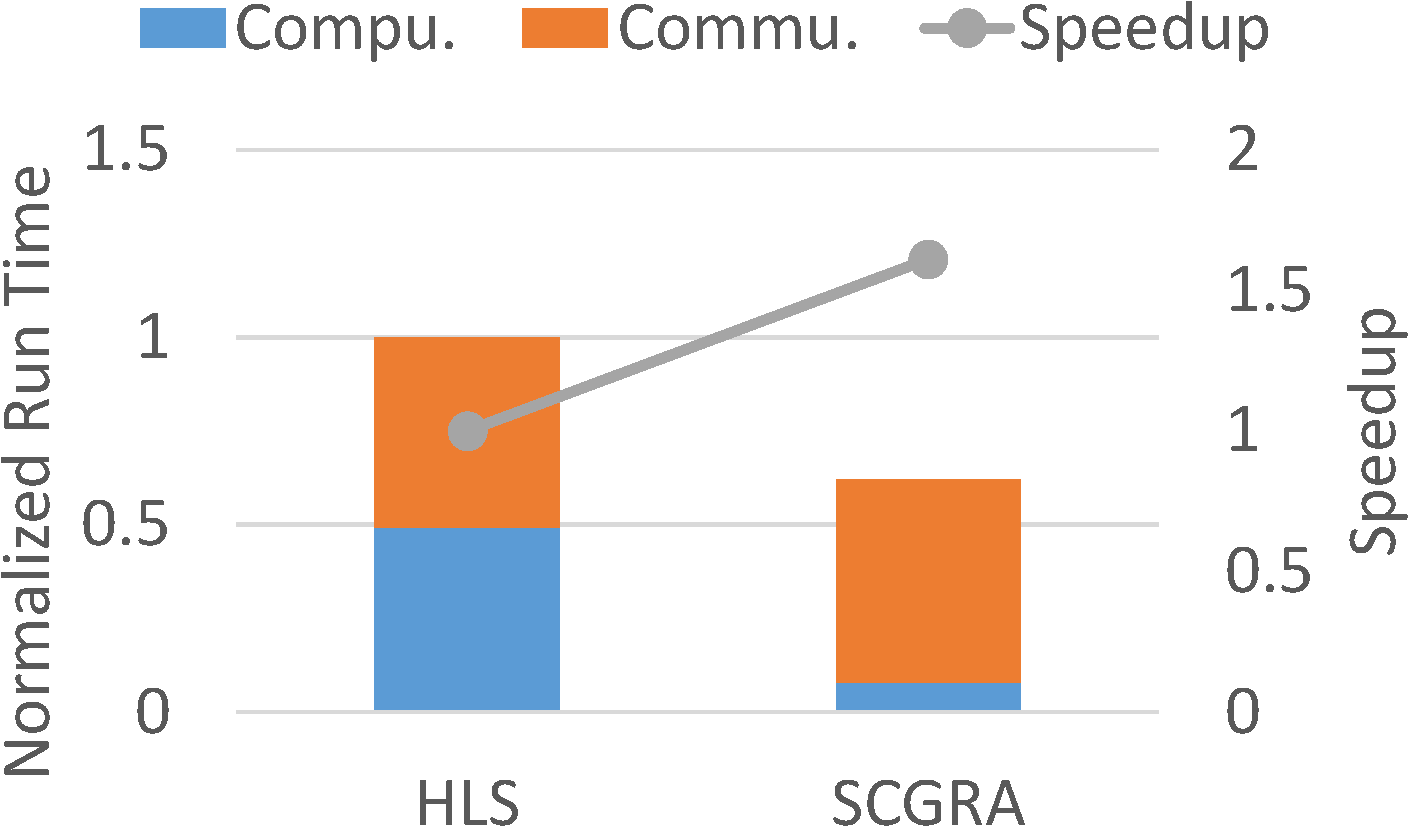
\includegraphics[width=0.22\textwidth]{km-hls-cp}
	}
    \caption{Performance comparison between the implementations 
        using HLS and the proposed automatic customization framework.
    All the run time is normalized to that of the HLS based implementations.}
	\label{fig:hls-cp}
\end{figure}


\figref{fig:hls-cp} shows the performance of the implementations using 
both design tools. The proposed customization framework utilizes 
SCGRA overlay as the backbone and it can't afford large 
BRAM for input/output buffers. As a result, the communication time is larger 
especially when there is a lot of data reuse between consecutive data transmission.
For instance, HLS based design can afford a 32k-word input buffer storing all 
the input data. However, the SCGRA overlay based design can only 
provide a 4k-word input buffer and it needs to transmit the same data 
multiple times to complete the matrix multiplication. Direct HLS can't support large 
loop unrolling due to the DSP resource constrain. SCGRA overlay based accelerator 
has a lot of distributed intermediate buffers and can accommodate larger loop unrolling.
Therefore, the accelerators generated using the proposed framework provides competitive 
pure computation time and overall performance especially for compute intensive loops.



\section{Related Work} \label{sec:relatedwork}
Despite of the performance and power advantages, the design 
productivity of developing FPGA applications remains low 
due to the lengthy compilation and complex application-specific 
customization. And it has become the major obstacle 
that hinders the wide adoption of FPGAs as commodity computing devices. 
The community from both the industry and academia have developed 
many different methods from diverse angles to tackle the problem. 
These methods can be roughly classified into three categories. 
The first category mainly focuses on improving the low-level 
implementation tools. A number of approaches such as making 
quality/runtime trade-offs \cite{mulpuri2001runtime}, parallel 
compilation \cite{moctar2014parallel, goeders2011deterministic, altera-pc, 
xilinx-pc} and using hard-macro techniques \cite{lavin2013improving, 
korf2011automatic} have been explored from this angle. The second 
category mainly centers the HLS design flow while the third one 
primarily relies on the overlay concept. They later two categories 
will be detailed in the following sections.

\subsection{High-Level Synthesis} 
With many years of continuous endeavor, a number of tools have emerged as 
mature solutions for HLS \cite{VivadoHLS, Legup, zhang2008autopilot}. They typically 
allow designers to express hardware designs using high-level  
description languages such as C, C++ etc. and also enable evaluation of different 
design choices using pragmas or directives. Indeed, they significantly improve 
the design productivity compared to the conventional hardware design flow using 
hardware description languages. However, when considering the overall design 
productivity of developing hybrid software-gateware applications, HLS is 
only addressing part of the problem, as the lengthy low-level compilation 
including synthesis, mapping, placing and routing remains a bottleneck for 
an application designer \cite{ROB2014, capalija2014tile}.

Customizing the generated hardware specifically to an user 
application is also time-consuming for designers and thus critical to the design 
productivity. A number of algorithms such as generic algorithms 
relied on local-search techniques \cite{schafer2009adaptive, 
sengupta1997genetic}, learning-based methods \cite{onlinecustomization, 
carrion2012machine}, divide and conquer algorithm \cite{DCcustomization} 
and a calibration free algorithm \cite{RCcustomization} etc. have been developed 
to perform the DSE on top of HLS tools. The algorithms can efficiently help automate the 
customization or DSE process. However, the algorithms must rely on HLS tools 
to estimate the implementation information such as implementation frequency, 
overhead or power for the corresponding customization. While the hardware generated 
can be irregular and may vary dramatically, thus the accuracy of the estimation 
especially on implementation frequency and power can be rather limited, which may
fail to optimize an HW/SW co-design problem.  

\subsection{Overlay Architectures}
Overlay architecture which is a virtual intermediate architecture overlaid on 
top of off-the-shelf FPGA is increasingly applied as a way to address the 
productivity challenge. 

Various overlays with diverse configuration granularities and flexibility 
ranging from virtual FPGAs \cite{Grant2011Malibu, ZUMA2012}, 
array-of-FUs \cite{mesh-FUs,ferreira2011fpga}, soft 
CGRA \cite{kissler2006dynamically, scgra-orig}, soft GPU \cite{Guppy2012GPU-Like}, 
vector processors\cite{Yiannacouras2009FPS, MXP2013} to 
configurable processors or multi-core processors \cite{unnikrishnan2009application, 
MARC2010, Yiannacouras2007Exploration, Capalija2009coarse-grain, OCTAVO2012, iDEA2012} 
have been developed over the years. SCGRA overlay provides unique 
advantages on compromising hardware implementation 
and performance for compute intensive nested loops as demonstrated 
by numerous ASIC CGRAs \cite{tessier2001reconfigurable, compton2002reconfigurable}.
Most importantly, it allows both rapid compilation by taking advantage of 
the overlays' tiling structure \cite{ROB2014} and efficient bitstream 
reuse within the design iterations of an application \cite{scgra-orig}, 
thus it is particularly promising for high productivity nested loop acceleration.

Despite of the promising potential, a complete automatic customization 
framework that enables application-specific optimization is still highly 
anticipated for the sake of design productivity and performance. 
The authors in \cite{colinheart} developed an SCGRA topology customization method 
using genetic algorithm and showed the potential benefits of the SCGRA 
overlay customization. However, the rest system design parameters such as 
on chip buffer size, loop unrolling factor etc. are not covered. 

Indeed, SCGRA overlays have many similarities in terms of array structure 
and scheduling algorithm with ASIC CGRAs. Nevertheless, ASIC CGRAs emphasize 
more on configuration capability and limited customization is allowed due 
to the overhead constraints \cite{zhou2014application, miniskar2014retargetable} 
while SCGRA overlays allow more intensive architectural customization 
because of the FPGA's inherent programmability. Moreover, hardware resources such as 
DSP blocks and RAM blocks available on FPGAs are discrete, which results in different 
design constraints for SCGRA overlay customization as well. 

By utilizing the SCGRA overlay as the backbone of the FPGA accelerator, 
a complete nested loop acceleration framework 
targeting CPU-FPGA system is developed. It supports intensive application-specific
customization including the overlay architectural customization, 
the compilation customization and communication interface customization 
for various design goals. When the customized design parameters are determined, 
corresponding hardware accelerator and software can be compiled to the target 
CPU-FPGA system rapidly eventually providing a push-button solution for a nested loop 
acceleration. 



\section{Conclusion} \label{sec:Conclusion}
In this work, we propose to replace the forward computing on GPPs with accelerator 
computing during training and have both the computing 
errors and the application data learned in the neural network models. 
In addition, we opt to protect critical neural layers to reduce the negative 
influence of computing errors.  
With the proposed resilient neural network training, 
the prediction accuracy of the retrained neural network models improves significantly 
when computing errors appear. 


%\appendix
%\section{Acknowledgement}

%\begin{acks}
%  The authors would like to thank Sam Ho for providing the suggestions on
%  HLS design debugging and optimization as well as the SDAccel usage. 

%\end{acks}


\bibliographystyle{plain}
\bibliography{refs}

%\balancecolumns
\end{document}

